\pdfminorversion=7
\documentclass[12pt,a4paper]{report}
\usepackage[a4paper,top=2.5cm,bottom=2.5cm,left=3cm,right=2.5cm]{geometry}
\usepackage[T1]{fontenc}
\usepackage[utf8]{inputenc}
\usepackage{lmodern,microtype,setspace,parskip,titlesec,titletoc,fancyhdr}
\usepackage{graphicx,float,caption,subcaption,booktabs,array,tabularx,longtable}
\usepackage{xcolor,listings,enumitem,amsmath,tcolorbox,mdframed,multirow,pifont,url,cite}
\usepackage{pdfpages,pdflscape,needspace}
\usepackage{hyperref}
\usepackage{tikz}
\usetikzlibrary{positioning,arrows.meta,shapes.geometric,fit,backgrounds,calc,shadows.blur}
\definecolor{kuBlue}{RGB}{0,56,101}
\definecolor{kuGold}{RGB}{197,151,51}
\definecolor{lightGray}{RGB}{245,245,245}
\definecolor{codeGray}{RGB}{248,248,248}
\definecolor{codeBorder}{RGB}{200,200,200}
\definecolor{linkBlue}{RGB}{0,90,160}
\hypersetup{colorlinks=true,linkcolor=linkBlue,citecolor=kuBlue,urlcolor=linkBlue,
pdftitle={Farm-to-Market Local Food Availability System},
pdfauthor={Abd Alrahman Ismaik, Ali Alshamsi, Mohammad Arwani},
pdfsubject={COSC444 Database Systems Lab B1},pdfkeywords={MySQL, Python, Tkinter, LangChain, inventory, loss and surplus}}
\titleformat{\chapter}[display]{\normalfont\huge\bfseries\color{kuBlue}}{\chaptertitlename\ \thechapter}{16pt}{\Huge}
\titlespacing{\chapter}{0pt}{-20pt}{20pt}
\titleformat{\section}{\normalfont\large\bfseries\color{kuBlue}}{\thesection}{1em}{}
\titlespacing{\section}{0pt}{14pt}{6pt}
\titleformat{\subsection}{\normalfont\normalsize\bfseries\color{kuBlue!80}}{\thesubsection}{1em}{}
\titlespacing{\subsection}{0pt}{10pt}{4pt}
\setlength{\headheight}{26pt}
\pagestyle{fancy}\fancyhf{}
\fancyhead[L]{\small\color{kuBlue}COSC444  |  Database Systems}
\fancyhead[R]{\small\color{kuBlue}Farm-to-Market | Lab B1}
\fancyfoot[C]{\small\thepage}
\renewcommand{\headrulewidth}{0.4pt}
\renewcommand{\footrulewidth}{0pt}
\renewcommand{\headrule}{\hbox to\headwidth{\color{kuBlue}\leaders\hrule height\headrulewidth\hfill}}
\fancypagestyle{plain}{\fancyhf{}\fancyfoot[C]{\small\thepage}\renewcommand{\headrulewidth}{0pt}}
\lstdefinestyle{projectCode}{backgroundcolor=\color{codeGray},basicstyle=\ttfamily\small,breaklines=true,breakatwhitespace=true,keepspaces=true,showstringspaces=false,frame=single,rulecolor=\color{codeBorder},xleftmargin=10pt,xrightmargin=10pt,aboveskip=6pt,belowskip=6pt,numberstyle=\tiny\color{gray},numbers=left,stepnumber=1,tabsize=4}
\lstset{style=projectCode}
\captionsetup{font={small,it},labelfont={bf,color=kuBlue},labelsep=period,margin=20pt,skip=6pt,hypcap=false}
\setcounter{tocdepth}{2}\setcounter{secnumdepth}{3}
\onehalfspacing
\setlength{\emergencystretch}{3em}
\begin{document}
\hypersetup{pageanchor=false}
\begin{titlepage}
\thispagestyle{empty}
{\color{kuBlue}\rule{\linewidth}{4pt}}\vspace{6pt}
{\color{kuGold}\rule{\linewidth}{1.5pt}}
\vspace{0.4cm}
\begin{center}
{\large\bfseries\color{kuBlue}Khalifa University}\\[4pt]
{\normalsize\color{gray}Department of Computer Science}\\[2pt]
{\normalsize\color{gray}COSC444 Database Systems  |  Fall 2026-2027  |  Lab B1}
\end{center}
\vspace{0.8cm}
\begin{center}
{\Huge\bfseries\color{kuBlue}Farm-to-Market}\\[10pt]
{\Large\color{kuGold}\bfseries Local Food Availability System}\\[10pt]
{\normalsize\color{gray}\itshape Technical Project Report}
\end{center}
\vspace{0.6cm}\hrule height 0.8pt\vspace{0.8cm}
\begin{minipage}[t]{0.48\linewidth}\centering
{\bfseries\color{kuBlue}Course Instructor}\\[6pt]
\begin{tabular}{@{}l@{}}Kamal Taha\\Associate Professor\\\texttt{kamal.taha@ku.ac.ae}\end{tabular}
\end{minipage}\hfill
\begin{minipage}[t]{0.48\linewidth}\centering
{\bfseries\color{kuBlue}Lab Instructors}\\[6pt]
\begin{minipage}{0.94\linewidth}
\begin{itemize}[leftmargin=1.2em,itemsep=3pt,topsep=0pt]
\item Nada Kawde
\item Ruosi Kong
\item Siniya Nedunkulathil
\end{itemize}
\end{minipage}
\end{minipage}
\vspace{0.8cm}\hrule height 0.8pt\vspace{0.6cm}
\begin{center}
{\bfseries\color{kuBlue}Project Team  |  Lab B1}\\[8pt]
\begin{tabular}{@{}ll@{}}\toprule
Abd Alrahman Ismaik & 100064692\\Ali Alshamsi & 100062530\\Mohammad Arwani & 100064908\\\bottomrule\end{tabular}
\end{center}
\vfill
\begin{center}\textbf{Prepared:} 19 November 2026\\\textbf{Target submission:} 19 November 2026\end{center}
\vspace{0.4cm}
{\color{kuGold}\rule{\linewidth}{1.5pt}}\vspace{4pt}
{\color{kuBlue}\rule{\linewidth}{4pt}}
\end{titlepage}
\pagenumbering{roman}
\hypersetup{pageanchor=true}
\chapter*{Abstract}\addcontentsline{toc}{chapter}{Abstract}
Farm-to-Market is an educational Python desktop application that models local produce availability through a MySQL database. Farmers record crop cycles, harvest lots, photos, reservations and stock dispositions; market buyers search supply, request quantities and record delivery receipts; administrators maintain reference data and assignments. Forecasts remain separate from harvested inventory, and stock is derived from dated movements with explicit units.

The implementation uses Tkinter, PyMySQL, Pillow and a read-only LangChain/Gemini assistant. Loss \& Surplus is the selected advanced feature. This report explains the database design, workflows and business rules with recorded verification evidence. It includes conceptual and relational diagrams, transaction rules, expected and observed test outcomes, and a concise summary of assistant validation.

The database records inventory changes as dated movements, retains product photos across restarts and links market requests to allocations and delivery receipts. The interface provides distinct farmer, market buyer and administrator workspaces. Donation eligibility follows the approved project policy: lots with a past sell-by date cannot be donated, while disposal remains available.

\textbf{Keywords:} relational database, MySQL, Python, Tkinter, inventory movements, transactions, LangChain, loss and surplus.
\clearpage\begingroup\small\setstretch{1.05}\tableofcontents\endgroup\clearpage
\pagenumbering{arabic}


\chapter{Project overview and architecture}

\Needspace{9\baselineskip}\section{Purpose and current result}
Farm-to-Market is a Python desktop prototype for local produce visibility. Farmers record crop cycles and harvest lots, buyers request supply and confirm receipts, and administrators maintain reference data. Operational data is fictional. The system does not represent national reserves or connect to government services. Loss \& Surplus is the selected advanced feature. [R1, R2]

The implemented workflows connect role-specific data entry with ownership checks, atomic transactions, movement-derived availability and persistent product photos. Requests may draw supply from multiple lots, and delivery receipts retain actual quantities and discrepancies. [R3-R6]


\begin{figure}[H]\centering
\resizebox{\linewidth}{!}{%
\begin{tikzpicture}[
box/.style={draw=kuBlue,fill=kuBlue!5,rounded corners,align=center,text width=4cm,minimum height=1.45cm,font=\small},
arr/.style={-{Latex[length=2mm]},thick,kuBlue}]
\node[box] (farmer) {\textbf{Farmer}\\Farm $\rightarrow$ cycle $\rightarrow$ lot\\$\rightarrow$ allocation $\rightarrow$ disposition};
\node[box,right=0.6cm of farmer] (buyer) {\textbf{Market Buyer}\\Search $\rightarrow$ request\\$\rightarrow$ track $\rightarrow$ receipt};
\node[box,right=0.6cm of buyer] (admin) {\textbf{Administrator}\\Users $\rightarrow$ assignments\\$\rightarrow$ reference data $\rightarrow$ audit};
\draw[arr] (farmer.north) -- ++(0,0.5cm) -| node[pos=0.25,above=2pt,font=\scriptsize]{supply} (buyer.north);
\node[draw=kuGold,thick,rounded corners,below=0.9cm of buyer,align=center,font=\small,fill=kuGold!8,text width=8.8cm,minimum height=0.9cm] (core) {Shared MySQL persistence: movements, allocations, receipts, BLOBs};
\draw[arr] (farmer.south) |- (core.west);
\draw[arr] (buyer.south) -- (core.north);
\draw[arr] (admin.south) |- (core.east);
\end{tikzpicture}}
\caption{Role workflows and shared persistence.}
\end{figure}
\Needspace{9\baselineskip}\section{Problem and role workflows}
The prototype models how local farms make harvested supply visible to markets, how buyers request it, and how reservations and delivery discrepancies affect stock. Its scope is the fictional sample dataset; no measured reduction in food waste or national supply-chain impact is claimed.

Farmers create farms and crop cycles, record harvests and photos, allocate assigned lots, and record loss, correction, donation or disposal. Buyers search produce, submit requests and confirm delivery quantities. Administrators maintain users, assignments and reference data and inspect operational history. Operational write permissions are checked in the data layer. [R2, R3]




\Needspace{5\baselineskip}\section{Application components}
\begin{figure}[H]\centering
\resizebox{\linewidth}{!}{%
\begin{tikzpicture}[
layer/.style={draw=kuBlue,fill=kuBlue!4,rounded corners,text width=8.5cm,minimum height=1.35cm,align=center,font=\small},
side/.style={draw=kuGold,fill=kuGold!6,rounded corners,text width=3.8cm,minimum height=1.5cm,align=center,font=\small},
arr/.style={-{Latex[length=2mm]},thick,kuBlue}]
\node[layer] (ui) {\textbf{Presentation Tier}  |  Tkinter/ttk desktop GUI (\path{app.py})\\Role tabs, forms, photo display, assistant worker};
\node[layer,below=0.75cm of ui] (logic) {\textbf{Business Logic Tier}  |  \path{db.py}\\Validation, ownership, parameterized SQL, transactions};
\node[layer,below=0.75cm of logic] (db) {\textbf{Persistence Tier}  |  MySQL 8.0\\15 tables, two views, stock movements, MEDIUMBLOB photos};
\node[side,right=0.75cm of logic] (ai) {\textbf{Assistant Tier}\\\path{assistant.py}\\LangChain/Gemini read-only};
\draw[arr] (ui) -- node[right,font=\scriptsize]{actions} (logic);
\draw[arr] (logic) -- node[right,font=\scriptsize]{PyMySQL / SQL} (db);
\draw[arr] (ui.east) -| node[pos=0.55,above,font=\scriptsize]{prompts} (ai.north);
\draw[arr] (ai.south) |- node[pos=0.7,below,font=\scriptsize]{read-only SQL} (db.east);
\end{tikzpicture}}
\caption{Four-tier application architecture.}
\end{figure}
The maintained entry point is \path{python app/app.py}. Tkinter/\allowbreak{}ttk handles the three role interfaces; \path{db.py} validates input, ownership and transactional SQL through PyMySQL; MySQL stores records and BLOB photos. \path{assistant.py} uses LangChain/\allowbreak{}Gemini for read-only questions. The demo-user selector supplies an identity for workflows; it is not password authentication. Shared search and assistant reads are not restricted to the selected user's own records. [R3]

The schema has 15 tables, 32 foreign keys, 13 named CHECK constraints and two derived views. An allocation links one lot to one request, allowing a request to draw on several lots and a lot to supply several requests. A receipt's UNIQUE allocation FK permits at most one receipt per allocation. \path{farm_users} resolves the many-to-many farmer assignment. Separate image and history tables retain multiple photos and dated changes. The lot's farm and crop are derived through its cycle. [R3, R6]

Reference tables reduce duplicate names and codes. The design deliberately repeats units and snapshots the promised quantity in receipts; application checks maintain cross-record consistency. SQL alone does not enforce equality of all related units, ownership, aggregate availability or all status-history values. [R3, R6]


The role configurations contain seven farmer tabs, five market-buyer tabs and six administrator tabs: eighteen role-tab entries, including shared search, assistant and review screens. These are not eighteen distinct screen classes.




\section{Source structure and submission files}
The application ZIP contains the maintained \path{app/} directory, root setup/run launchers, README, poster and integrity manifest. Table~\ref{tab:runtime-files} maps runtime/configuration files to their responsibilities; Table~\ref{tab:support-files} covers the remaining delivered assets and verification sources. This technical report and its editable LaTeX bundle are separate deliverables from the application ZIP.

\begingroup\footnotesize\setstretch{1.1}\setlength{\tabcolsep}{3pt}
\begin{longtable}{>{\raggedright\arraybackslash}p{0.40\linewidth}>{\raggedright\arraybackslash}p{0.55\linewidth}}
\caption{Application code, configuration and launch files.}\label{tab:runtime-files}\\\toprule
\textbf{File} & \textbf{Role}\\\midrule\endfirsthead
\toprule\textbf{File} & \textbf{Role}\\\midrule\endhead
\bottomrule\endlastfoot
\path{README.md} & Project overview, prerequisites, package installation, configuration, setup and launch instructions.\\[4pt]
\path{app/.env.example} & Configuration template with database connection fields and Gemini settings; replace placeholders locally.\\[4pt]
\path{app/app.py} & Tkinter/ttk entry point, role tabs, forms, tables, image widgets, feedback messages and assistant worker.\\[4pt]
\path{app/assistant.py} & LangChain/Gemini query generation, schema/SQL validation, read-only execution and answer summarization.\\[4pt]
\path{app/check_database.py} & Database connection preflight; returns a status used by the Windows launcher.\\[4pt]
\path{app/db.py} & PyMySQL connections, parameterized queries, input and ownership validation, stock calculations and transactional business operations.\\[4pt]
\path{app/requirements.txt} & Lists the six third-party Python dependencies installed during setup.\\[4pt]
\path{app/run.bat} & Selects project Python when available, checks imports and database connectivity, then starts the GUI.\\[4pt]
\path{app/schema.sql} & Creates and populates farm\_market\_db, including tables, keys, constraints, derived views and BLOB sample photos.\\[4pt]
\path{app/setup.bat} & Installs requirements and runs the database initializer.\\[4pt]
\path{app/setup_database.py} & Creates a local configuration when missing and executes the schema/population script.\\[4pt]
\path{run.bat} & Root Windows launcher; delegates to the application launcher.\\[4pt]
\path{setup.bat} & Root first-time setup launcher; delegates to application setup.\\[4pt]
\end{longtable}\endgroup
\begingroup\footnotesize\setstretch{1.1}\setlength{\tabcolsep}{3pt}
\begin{longtable}{>{\raggedright\arraybackslash}p{0.40\linewidth}>{\raggedright\arraybackslash}p{0.55\linewidth}}
\caption{Images, verification sources and delivery artifacts.}\label{tab:support-files}\\\toprule
\textbf{File} & \textbf{Role}\\\midrule\endfirsthead
\toprule\textbf{File} & \textbf{Role}\\\midrule\endhead
\bottomrule\endlastfoot
\path{MANIFEST.md} & SHA-256 inventory of the application ZIP payload for file-integrity checks.\\[4pt]
\path{app/sample_images/bell_pepper.jpg} & External bell-pepper image supplied for photo-upload demonstrations.\\[4pt]
\path{app/sample_images/cucumber.jpg} & External cucumber image supplied for photo-upload demonstrations.\\[4pt]
\path{app/sample_images/eggplant.jpg} & External eggplant image supplied for photo-upload demonstrations.\\[4pt]
\path{app/sample_images/zucchini.jpg} & External zucchini image supplied for photo-upload demonstrations.\\[4pt]
\path{app/tests/check_assistant_readonly.py} & Checks assistant/read-only behavior and compares the database state.\\[4pt]
\path{app/tests/test_business_rules.py} & Original scripted business-rule checks using a disposable database.\\[4pt]
\path{app/tests/test_validation_support.py} & Checks output-directory guards used by the verification helpers.\\[4pt]
\path{app/tests/track_a_gui_flow.py} & Scripted GUI workflow and fresh-process photo-persistence checks.\\[4pt]
\path{app/tests/track_a_remaining_checks.py} & Extended database, ownership, image, boundary, rollback and concurrent-operation checks.\\[4pt]
\path{app/tests/validation_support.py} & Shared command-line and safe-output-path helpers for verification scripts.\\[4pt]
\path{submission/COSC444_Farm-to-market_Poster.pdf} & Project poster in PDF format.\\[4pt]
\end{longtable}\endgroup
\section{Libraries and runtime requirements}
Python with Tcl/Tk and a running MySQL 8 server provide the local runtime. The six pip dependencies are declared in \path{app/requirements.txt}. Their installed code is not bundled in the application ZIP: setup downloads and installs them. Tkinter is supplied with a Tcl/Tk-enabled Python installation, while MySQL is installed and started separately.

\begingroup\small\setstretch{1.1}\setlength{\tabcolsep}{3pt}
\begin{longtable}{>{\raggedright\arraybackslash}p{0.32\linewidth}>{\raggedright\arraybackslash}p{0.63\linewidth}}
\caption{Libraries and their technical roles.}\\\toprule
\textbf{Library or runtime} & \textbf{Use in the application}\\\midrule\endfirsthead
\toprule\textbf{Library or runtime} & \textbf{Use in the application}\\\midrule\endhead\bottomrule\endlastfoot
Tkinter/ttk & Desktop window, themed controls, notebooks, forms, dialogs and table views.\\[4pt]
\path{pymysql} & MySQL connections, dictionary cursors, parameter binding, commit and rollback.\\[4pt]
\path{cryptography} & Cryptographic support for MySQL authentication through PyMySQL.\\[4pt]
\path{python-dotenv} & Loads local database and Gemini configuration from \path{app/.env}.\\[4pt]
\path{pillow} & Verifies and decodes JPEG/PNG data; bridges stored image bytes to Tkinter display objects.\\[4pt]
\path{langchain-core} & Builds prompt, model and text-output chains used for SQL generation and summaries.\\[4pt]
\path{langchain-google-genai} & Connects the LangChain model calls to Google Gemini.\\[4pt]
MySQL 8 & Stores relational records, BLOB photos, constraints, views and transaction state.\\[4pt]
\end{longtable}\endgroup

\section{How the code layers cooperate}
A Tkinter form collects input and calls a function in \path{db.py}. That function parses dates/quantities, checks the selected user's ownership and validates the requested operation. Related SQL writes execute within the transaction context, which commits on success and rolls back on exception. The GUI refreshes its tables from database queries and shows a friendly result message.

For photos, Pillow validates the selected file before \path{db.py} inserts its binary data into MySQL. When a lot is selected later, the GUI retrieves those bytes and creates an image widget. This database-backed path preserves the photo across application restarts.

For assistant questions, a background thread runs the LangChain generation step using an allowlisted schema. The candidate query is validated and executed in a read-only MySQL transaction. A second chain summarizes the returned records. The worker queues its result for the Tkinter main thread, which updates the answer, SQL and supporting-record widgets. Clarification, unsupported requests and provider errors follow the same result-display path.

\section{Setup and execution on a new machine}
\begin{enumerate}[leftmargin=1.5em,itemsep=4pt]
\item Extract the application ZIP. Install Python with Tcl/Tk and MySQL 8, then start the intended MySQL server. Confirm \path{python --version} and \path{python -m tkinter} work.
\item Run root \path{setup.bat}. It installs \path{app/requirements.txt}; \path{setup_database.py} prompts for database settings and creates \path{app/.env} when absent, then executes \path{app/schema.sql}. Initialization drops and recreates \path{farm_market_db}; use it when initialization or reset is intended.
\item Add a Gemini API key to \path{app/.env} to enable live assistant responses. Other workflows use MySQL directly. Configure the accessible model through \path{GEMINI_MODEL}.
\item Run root \path{run.bat}. The launcher checks dependencies and database connectivity before opening the GUI. A failed connection offers retry after the configured server is started. Alternatively run \path{python app/app.py} from the extracted root.
\end{enumerate}

The configuration fields are \path{DB_HOST}, \path{DB_PORT}, \path{DB_USER}, \path{DB_PASSWORD}, \path{DB_NAME}, \path{GEMINI_API_KEY} and \path{GEMINI_MODEL}. The SQL initializer targets \path{farm_market_db}; changing \path{DB_NAME} alone does not change its reset target. Real \path{.env} settings and local virtual environments are excluded from the ZIP. The verification scripts are optional and operate on an intended disposable database; they are not part of normal startup.

\chapter{Database design and business rules}

\section{Enforcement of business rules}


\begingroup\small\setstretch{1.12}\setlength{\tabcolsep}{3pt}
\begin{longtable}{>{\raggedright\arraybackslash}p{0.1\linewidth}>{\raggedright\arraybackslash}p{0.28\linewidth}>{\raggedright\arraybackslash}p{0.54\linewidth}}
\caption{Business rules and enforcement responsibilities}\\\toprule
\textbf{Rule} & \textbf{Requirement} & \textbf{Database and application responsibilities} \\ \midrule
\endfirsthead
\toprule
\textbf{Rule} & \textbf{Requirement} & \textbf{Database and application responsibilities} \\ \midrule
\endhead
\midrule\multicolumn{3}{r}{\small Continued on next page}\\\endfoot
\bottomrule\endlastfoot
BR-01 & Farm, cycle and lot links & FKs link cycles to farms and lots to cycles. Harvest checks validate assigned farm, dates, status and unit. \\[4pt]
BR-02 & Separate forecasts & Expected quantity stays in \path{crop_cycles}. \path{stock_summary()} calculates remaining expected harvest separately; it is a Python function, not a SQL view. \\[4pt]
BR-03 & Movement-derived stock & \path{v_lot_stock} derives balances from movements. SQL rejects zero quantities and negative non-correction movements; application writes preserve workflow consistency. \\[4pt]
BR-04 & Partial, atomic allocation & Positive allocation quantity and FKs are constrained in SQL. Locked application transactions check crop/\allowbreak{}unit match, request remainder, ownership and availability. \\[4pt]
BR-05 & Record receipt shortfalls & One UNIQUE allocation reference per receipt; SQL checks quantity bounds and discrepancy arithmetic. Application records delivery, release and loss together. \\[4pt]
BR-06 & Explicit units & Quantity records reference units; crops use \path{default_unit_id}. Application enforces related-unit equality and keeps aggregates separated by unit. No conversion is implemented. \\[4pt]
BR-07 & Ownership of writes & Farm assignments use the \path{farm_users} junction and buyer users link to markets. Application role/\allowbreak{}ownership checks restrict operational writes. Shared reads remain visible. \\[4pt]
BR-08 & History and deactivation & Movements and request-history rows retain responsible users and dates, with reasons where applicable. Supported reference records are deactivated; not every table has \path{is_active}. \\[4pt]
BR-09 & Photos linked to lots & Image FKs and MIME checks complement application size/\allowbreak{}type/\allowbreak{}decode checks. The GUI handles unavailable or corrupt images. \\[4pt]
BR-10 & Fictional operational data & Seed accounts and operational records are fictional. This is a data-selection policy, not a SQL constraint that can establish the truth of every record. \\[4pt]
\end{longtable}\endgroup

\section{Schema summary}

The SQL contains fifteen tables, thirty-two foreign keys, thirteen named CHECK constraints and two views. Full column types and relationships appear in the relational appendix; \path{app/schema.sql} is the executable creation and population source. SQL does not enforce every cross-record business rule. [R3]



\begingroup\small\setstretch{1.12}\setlength{\tabcolsep}{3pt}
\begin{longtable}{>{\raggedright\arraybackslash}p{0.24\linewidth}>{\raggedright\arraybackslash}p{0.7\linewidth}}
\caption{All fifteen physical tables}\\\toprule
\textbf{Table} & \textbf{Purpose and key relationships} \\ \midrule
\endfirsthead
\toprule
\textbf{Table} & \textbf{Purpose and key relationships} \\ \midrule
\endhead
\midrule\multicolumn{2}{r}{\small Continued on next page}\\\endfoot
\bottomrule\endlastfoot
\path{emirates} & Location reference; unique emirate name. \\[4pt]
\path{units} & Measurement reference; unique code, display name and active flag. \\[4pt]
\path{crops} & Crop reference with a default unit and active flag. \\[4pt]
\path{markets} & Buyer-market reference linked to an emirate. \\[4pt]
\path{farms} & Farm reference linked to an emirate. \\[4pt]
\path{users} & Demo identities, role and optional market. Market users must have a market; other roles must not. \\[4pt]
\path{farm_users} & Composite farm/\allowbreak{}user key resolves farmer assignments to multiple farms. \\[4pt]
\path{crop_cycles} & Farm, crop, unit and creator; planting/\allowbreak{}expected dates and forecast quantity. \\[4pt]
\path{harvest_lots} & Cycle, unit and creator; quantity harvested, harvest date, optional sell-by and active flag. \\[4pt]
\path{harvest_lot_images} & Lot and uploader; filename, MIME type, upload time and MEDIUMBLOB data. \\[4pt]
\path{market_requests} & Market, crop, unit and creator; requested quantity, needed-by date and status. \\[4pt]
\path{request_status_history} & Request and responsible user; old/\allowbreak{}new status, timestamp and reason. \\[4pt]
\path{allocations} & Request, lot, unit and allocating user; quantity, status and allocation date. \\[4pt]
\path{delivery_receipts} & Unique allocation, unit and confirming user; promised/\allowbreak{}received/\allowbreak{}discrepancy quantities, reason and dates. \\[4pt]
\path{stock_movements} & Lot, unit, responsible user and optional allocation; movement type, signed correction or positive quantity, date and reason. \\[4pt]
\end{longtable}\endgroup


\begingroup\small\setstretch{1.12}\setlength{\tabcolsep}{3pt}
\begin{longtable}{>{\raggedright\arraybackslash}p{0.28\linewidth}>{\raggedright\arraybackslash}p{0.13\linewidth}>{\raggedright\arraybackslash}p{0.51\linewidth}}
\caption{Foreign-key and CHECK-constraint inventory}\\\toprule
\textbf{Table} & \textbf{Foreign keys} & \textbf{Named CHECK constraints} \\ \midrule
\endfirsthead
\toprule
\textbf{Table} & \textbf{Foreign keys} & \textbf{Named CHECK constraints} \\ \midrule
\endhead
\midrule\multicolumn{3}{r}{\small Continued on next page}\\\endfoot
\bottomrule\endlastfoot
\path{emirates} & 0 & None \\[4pt]
\path{units} & 0 & None \\[4pt]
\path{crops} & 1 & None \\[4pt]
\path{markets} & 1 & None \\[4pt]
\path{farms} & 1 & None \\[4pt]
\path{users} & 1 & \path{chk_user_market} \\[4pt]
\path{farm_users} & 2 & None \\[4pt]
\path{crop_cycles} & 4 & \path{chk_cycle_qty}, \path{chk_cycle_dates} \\[4pt]
\path{harvest_lots} & 3 & \path{chk_lot_qty}, \path{chk_lot_sell_by} \\[4pt]
\path{harvest_lot_images} & 2 & \path{chk_img_type} \\[4pt]
\path{market_requests} & 4 & \path{chk_req_qty} \\[4pt]
\path{request_status_history} & 2 & None \\[4pt]
\path{allocations} & 4 & \path{chk_alloc_qty} \\[4pt]
\path{delivery_receipts} & 3 & \path{chk_rcpt_nonneg}, \path{chk_rcpt_max}, \path{chk_rcpt_diff} \\[4pt]
\path{stock_movements} & 4 & \path{chk_mov_nonzero}, \path{chk_mov_sign} \\[4pt]
\end{longtable}\endgroup

The views are \path{v_lot_stock} and \path{v_request_status}. Reference tables reduce duplicate names and codes. Units are deliberately repeated in transaction records, while receipt quantities preserve the promised amount at settlement. The report does not claim a formal normalization proof from table counts alone.


\begin{figure}[H]\centering
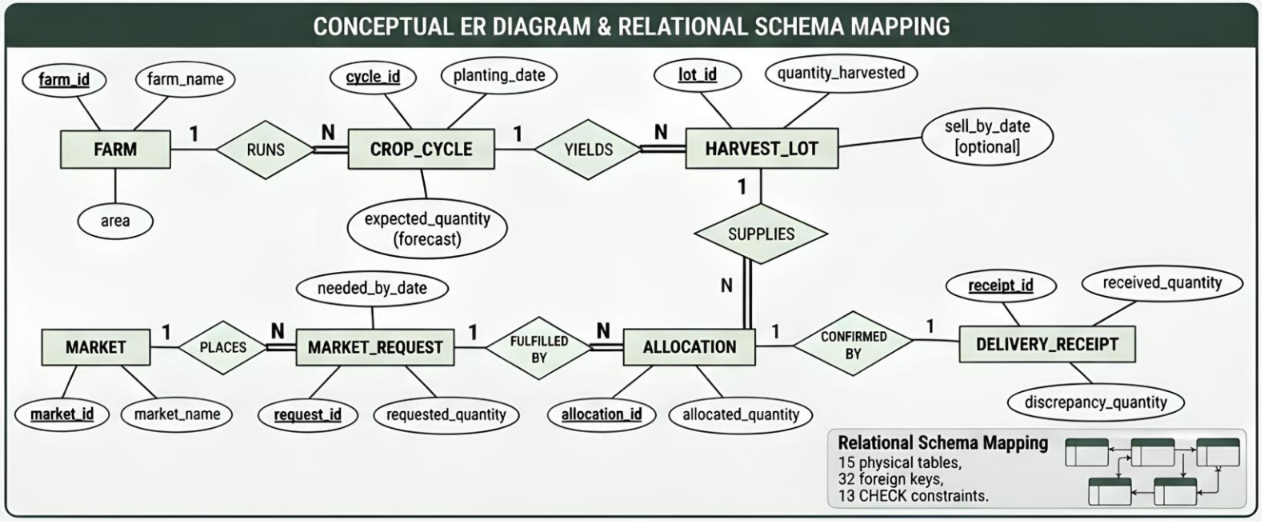
\includegraphics[width=\linewidth,height=0.34\textheight,keepaspectratio]{figures/operational-overview.png}
\caption{Simplified relational overview of operational entities.}
\label{fig:operational-overview}
\end{figure}
The overview highlights the main supply-to-receipt chain. Its receipt link is simplified: an allocation has zero or one receipt before settlement. The complete conceptual and relational sheets in the appendices retain the detailed model.

\Needspace{12\baselineskip}\section{Seed coverage}


\begingroup\small\setstretch{1.12}\setlength{\tabcolsep}{3pt}
\begin{longtable}{>{\raggedright\arraybackslash}p{0.43\linewidth}>{\raggedright\arraybackslash}p{0.24\linewidth}>{\raggedright\arraybackslash}p{0.25\linewidth}}
\caption{Required and supplied sample data}\\\toprule
\textbf{Record category} & \textbf{Required minimum} & \textbf{SQL seed count} \\ \midrule
\endfirsthead
\toprule
\textbf{Record category} & \textbf{Required minimum} & \textbf{SQL seed count} \\ \midrule
\endhead
\midrule\multicolumn{3}{r}{\small Continued on next page}\\\endfoot
\bottomrule\endlastfoot
Farms & 3 & 4 \\[4pt]
Markets & 4 & 4 \\[4pt]
Crops & 5 & 6 \\[4pt]
Crop cycles & 8 & 10 \\[4pt]
Harvest lots & 12 & 13 \\[4pt]
Stock movements & 15 & 38 \\[4pt]
Market requests & 8 & 9 \\[4pt]
Delivery receipts & 6 & 6 \\[4pt]
Product images & Required; no numeric minimum & 12 BLOB records; four external upload examples \\[4pt]
\end{longtable}\endgroup

These are the supplied seed counts, also observed in the historical DB-01b audit. They do not describe today's mutable demo database. Seed dates are relative to setup date. [R2, R6]


\chapter{Inventory and transactions}

\Needspace{9\baselineskip}\section{Stock and forecasts}
\path{v_lot_stock} derives stock from dated movements. All movement quantities are positive except signed CORRECTION. Each quantity has an explicit unit; kg, boxes and crates are never silently added or converted. [BR-02, BR-03, BR-06 in R2]

\begin{lstlisting}
on_hand = harvest + signed correction - delivered - loss - donated - disposed
reserved = reserved movements - released reservations - delivered
available = on_hand - reserved
\end{lstlisting}
\Needspace{181pt}
\begingroup\small\setstretch{1.12}\setlength{\tabcolsep}{3pt}
\begin{longtable}{>{\raggedright\arraybackslash}p{0.4\linewidth}>{\raggedright\arraybackslash}p{0.17\linewidth}>{\raggedright\arraybackslash}p{0.17\linewidth}>{\raggedright\arraybackslash}p{0.18\linewidth}}
\caption{Stock lifecycle under the receipt-shortfall policy}\\\toprule
\textbf{Event on one 100 kg lot} & \textbf{On hand} & \textbf{Reserved} & \textbf{Available} \\ \midrule
\endfirsthead
\toprule
\textbf{Event on one 100 kg lot} & \textbf{On hand} & \textbf{Reserved} & \textbf{Available} \\ \midrule
\endhead
\midrule\multicolumn{4}{r}{\small Continued on next page}\\\endfoot
\bottomrule\endlastfoot
Harvest 100 kg & 100 & 0 & 100 \\[4pt]
Allocate 30 kg & 100 & 30 & 70 \\[4pt]
Receive 25 kg; release 5 kg; record 5 kg loss & 70 & 0 & 70 \\[4pt]
\end{longtable}\endgroup
The last row is current shortfall policy, observed by Track A DEL-02. A release without delivery returns the second row to 100/\allowbreak{}0/\allowbreak{}100. Forecast remains in \path{crop_cycles}: remaining expected quantity is max(expected minus harvested, 0) for non-completed cycles, separate from available stock. [R3, R6]


\Needspace{210pt}
\begingroup\small\setstretch{1.12}\setlength{\tabcolsep}{3pt}
\begin{longtable}{>{\raggedright\arraybackslash}p{0.4\linewidth}>{\raggedright\arraybackslash}p{0.17\linewidth}>{\raggedright\arraybackslash}p{0.17\linewidth}>{\raggedright\arraybackslash}p{0.18\linewidth}}
\caption{Movement sequence within one atomic receipt transaction}\\\toprule
\textbf{Sequential receipt step} & \textbf{On hand} & \textbf{Reserved} & \textbf{Available} \\ \midrule
\endfirsthead
\toprule
\textbf{Sequential receipt step} & \textbf{On hand} & \textbf{Reserved} & \textbf{Available} \\ \midrule
\endhead
\midrule\multicolumn{4}{r}{\small Continued on next page}\\\endfoot
\bottomrule\endlastfoot
After 100 kg harvest and 30 kg reservation & 100 & 30 & 70 \\[4pt]
Record 25 kg delivered & 75 & 5 & 70 \\[4pt]
Release the remaining 5 kg reservation & 75 & 0 & 75 \\[4pt]
Record 5 kg shortfall as loss & 70 & 0 & 70 \\[4pt]
\end{longtable}\endgroup

Intermediate rows explain the arithmetic inside one transaction. They are not separate committed states. The allocation is settled by this receipt; a later top-up receipt is not supported.


\Needspace{9\baselineskip}\section{Atomic writes and ownership}
Values use parameterized SQL. A transaction commits on success, rolls back on exception and closes its connection. \path{get_connection} uses READ COMMITTED; write paths lock the parent request before its allocations and lock affected lots in stable order. The dated follow-up exercised competing allocations, loss/\allowbreak{}correction, same-request releases and partial receipts. See the dated before/\allowbreak{}after results in the testing chapter. [R3, R6]

\Needspace{239pt}
\begingroup\small\setstretch{1.12}\setlength{\tabcolsep}{3pt}
\begin{longtable}{>{\raggedright\arraybackslash}p{0.24\linewidth}>{\raggedright\arraybackslash}p{0.7\linewidth}}
\caption{Transactional checks and related writes}\\\toprule
\textbf{Operation} & \textbf{Checks and records in the transaction} \\ \midrule
\endfirsthead
\toprule
\textbf{Operation} & \textbf{Checks and records in the transaction} \\ \midrule
\endhead
\midrule\multicolumn{2}{r}{\small Continued on next page}\\\endfoot
\bottomrule\endlastfoot
Harvest & Lock cycle; check assigned farm, status, dates and unit. Insert lot, HARVEST\_\allowbreak{}ADDED movement and optional validated BLOB; update cycle to HARVESTING. \\[4pt]
Allocate & Lock request, then lot; check farmer ownership, crop/\allowbreak{}unit equality, request remainder and available stock. Insert allocation and RESERVED movement; update status/\allowbreak{}history. \\[4pt]
Release or cancel & Check owner and current status. Release reservations and update allocation/\allowbreak{}request status and history together. Cancellation after a receipt is refused. \\[4pt]
Confirm delivery & Check buyer's market and reserved allocation. Insert unique receipt, delivered quantity, release/\allowbreak{}loss for shortfall; settle allocation and update request/\allowbreak{}history. \\[4pt]
Loss or disposition & Farmer must own the lot; require reason and quantity within availability. Donation is rejected if recorded sell-by is before database \path{CURDATE()}; disposal remains available. Record actor, date and movement. \\[4pt]
\end{longtable}\endgroup
\Needspace{9\baselineskip}\section{Database constraints and application checks}
SQL enforces PK/\allowbreak{}FK/\allowbreak{}UNIQUE constraints, enumerated domains, positive lot/\allowbreak{}request/\allowbreak{}allocation quantities, nonnegative forecasts/\allowbreak{}receipts, receipt bounds and discrepancy arithmetic. CHECK constraints require sensible cycle and sell-by dates and a market link only for buyers. Application logic adds active-reference checks, role/\allowbreak{}record ownership, matching units, finite quantities with at most two decimal places, current-date rules and stock/\allowbreak{}remainder checks. Reference data is deactivated to preserve history. [R3, R6]

\Needspace{9\baselineskip}\section{Images and role interfaces}
Farmers upload JPEG/\allowbreak{}PNG files of up to 5 MiB. Bytes, filename, MIME type, uploader and timestamp are stored in \path{harvest_lot_images} as MEDIUMBLOB data. Buyers retrieve photos by lot, including after restart. Upload validation verifies and fully decodes image bytes before storage; the interface handles unavailable or corrupt images with a fallback state. [R3-R6]

\Needspace{9\baselineskip}\section{Loss and Surplus}
Active lots with available stock above zero are candidates. Priority is expired, then near expiry, then currently unallocated ageing stock. Defaults are 3 expiry days and 7 surplus days; inclusive whole-number ranges are 0-60 and 0-365. Expired means sell-by before today; near expiry includes sell-by today through the selected threshold; surplus requires age at least the threshold and no non-RELEASED allocation. Query thresholds are not persisted settings. [R3, R6]

Donation and disposal each reduce on-hand and available equally, leave reservations unchanged, and record actor/\allowbreak{}date/\allowbreak{}reason. Farmers act only on assigned lots; administrators inspect history without operational controls. The approved project policy rejects donation after the recorded sell-by date and permits disposal. In-date and undated lots may be donated subject to stock and ownership checks. The original proposal requires two disposition actions but does not set donation eligibility; it defines sell-by as the recommended last date for sale. This conservative application policy is not a food-safety determination. [R2]

\Needspace{9\baselineskip}\section{Current application policies}
DELIVERED uses settled allocated totals, not actual received totals: seed request \#6 is 60 allocated/\allowbreak{}52 received. One receipt finalizes an allocation and turns shortfall into loss; there is no later top-up receipt. The GUI's ``approved correction'' is a farmer action with a required reason and no administrator approval step. Released historical allocations do not disqualify surplus. These are documented project policy choices, not instructor requirements or endorsements. Donation eligibility blocks past-sell-by lots; in-date or undated lots may be donated.  [R6]


\chapter{Assistant and error handling}

\Needspace{9\baselineskip}\section{Assistant execution boundary}
The GUI uses a background worker. The assistant supplies an allowlisted non-BLOB schema, asks Gemini for SELECT/\allowbreak{}CTE or clarification/\allowbreak{}refusal, applies regex checks and a 200-row result cap, then executes \path{START TRANSACTION READ ONLY} and rolls back. A second chain summarizes only the first 50 rows. SQL and supporting records are visible. Generated queries pass schema and SQL checks before execution. Shared assistant reads are available across the demo roles. The recorded direct write attempt was rejected by MySQL error 1792. [R3-R5]


The recorded assistant validation covered supported questions, clarification, unsupported data, protected-data refusal and empty results, including a direct write attempt. Fourteen questions were compared with separately written reference SQL in dated evidence. The interface displays supporting records so users can inspect the basis of each answer. [R5]

\Needspace{9\baselineskip}\section{Errors and startup}
Database exceptions are translated into short user messages for connection failure, rejected credentials, missing database, duplicates, invalid references and other expected failures. Form validation handles invalid dates, quantities, units and empty inputs. Transaction failures roll back related writes. [R3]

The November 19 launcher preflight checks the configured database before opening the GUI and offers retry on failure. On the original PC only, a refused connection to \path{127.0.0.1:3307} can invoke the ignored local demo-start helper when present. A new device needs its own MySQL installation, credentials and initial setup.  [R9]

Setup executes \path{DROP DATABASE IF EXISTS farm_market_db}. Relaunching preserves database records and BLOB images; setup recreates the seed database. Changing \path{DB_NAME} alone does not retarget setup. A Gemini key and internet access are needed for live assistant answers. The recorded model's availability can vary by account and date. [R3, R5]


\chapter{Graphical user interface}\begingroup\small\setstretch{1.12}\setlength{\intextsep}{8pt}
The Tkinter interface organizes work into role-specific tabs with shared search and assistant screens. Tables display explicit units and quantities; action buttons open forms or apply the selected operation. Product photos appear beside the associated lot, while messages confirm saved actions or explain invalid input.

The figures illustrate the application's main screens using fictional demo data. Operational screenshots are preserved validation captures from November 16-17, 2026; the administrator view was captured on November 19. Displayed rows and dates describe those captures. [R4-R6, R10]

\section{User selection and navigation}
Users choose a named farmer, market buyer or administrator to enter the corresponding workspace. Farmer cards identify assigned farms, buyer cards identify the market, and the header retains the selected identity. Switch user returns to this screen. The selector supplies a demo identity; it is not password authentication.
\begin{figure}[H]\centering
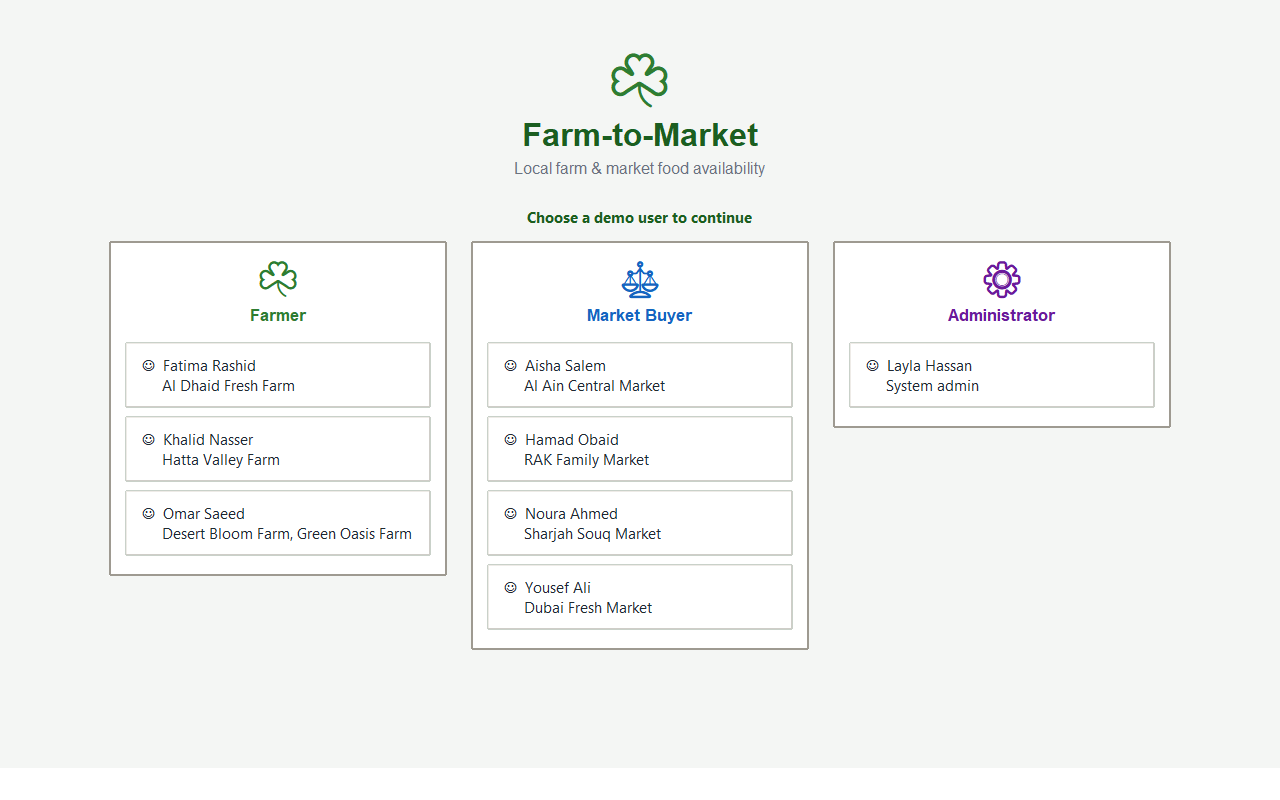
\includegraphics[width=\linewidth,height=.43\textheight,keepaspectratio]{figures/gui/selector.png}
\caption{Demo-user selection grouped by role.}
\label{gui:selector}
\end{figure}
\clearpage
\section{Farmer workspace}
\textbf{Harvest and Stock.} The upper summary separates expected harvest from on-hand, reserved and available quantities. Selecting a lot shows its stored photo; controls support harvest entry, photo upload, loss/correction and movement history.
\begin{figure}[H]\centering
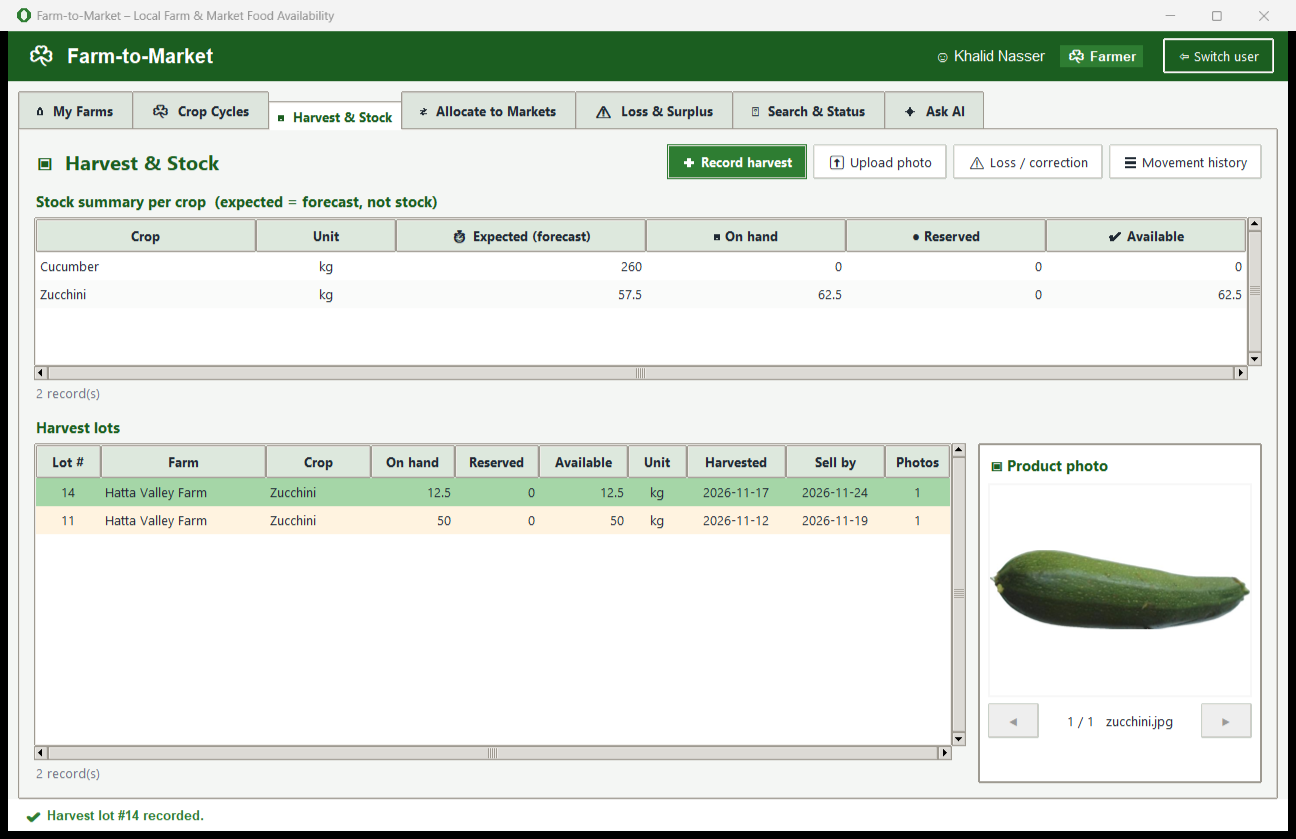
\includegraphics[width=\linewidth,height=.32\textheight,keepaspectratio]{figures/gui/harvest.png}
\caption{Farmer stock summary, harvest lots and product photo.}
\label{gui:harvest}
\end{figure}
\textbf{Allocate to Markets.} Open requests appear beside matching lots of the same crop and unit. The farmer enters an allocation quantity; the lower table retains reservations and their status. The capture shows saved reservations after allocation.
\begin{figure}[H]\centering
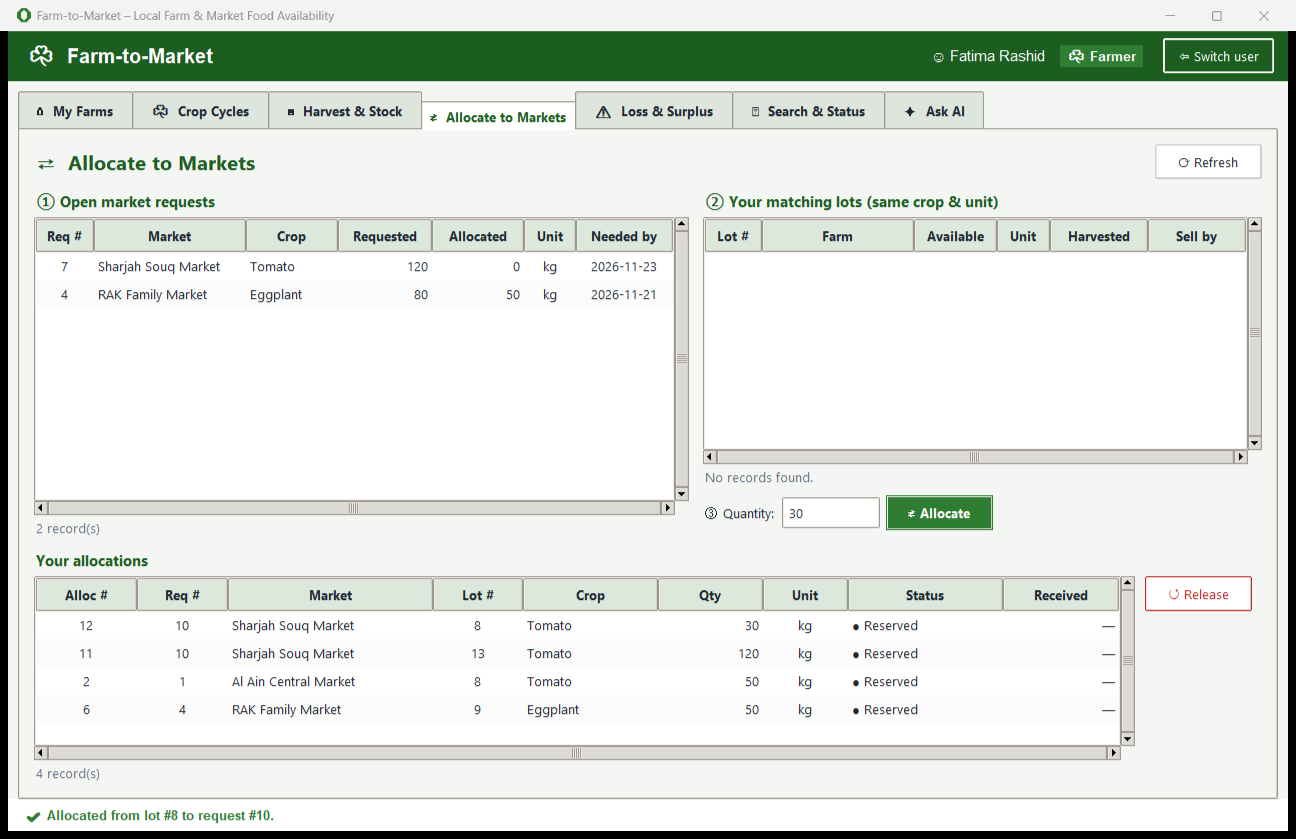
\includegraphics[width=\linewidth,height=.32\textheight,keepaspectratio]{figures/gui/allocation.png}
\caption{Farmer allocation screen and reserved allocations.}
\label{gui:allocation}
\end{figure}
\clearpage
\section{Market buyer workspace}
\textbf{Find Produce.} Crop, emirate, quantity and date filters narrow available supply. Selecting a lot displays its photo. Request this crop opens the request form; My Requests provides subsequent status tracking.
\begin{figure}[H]\centering
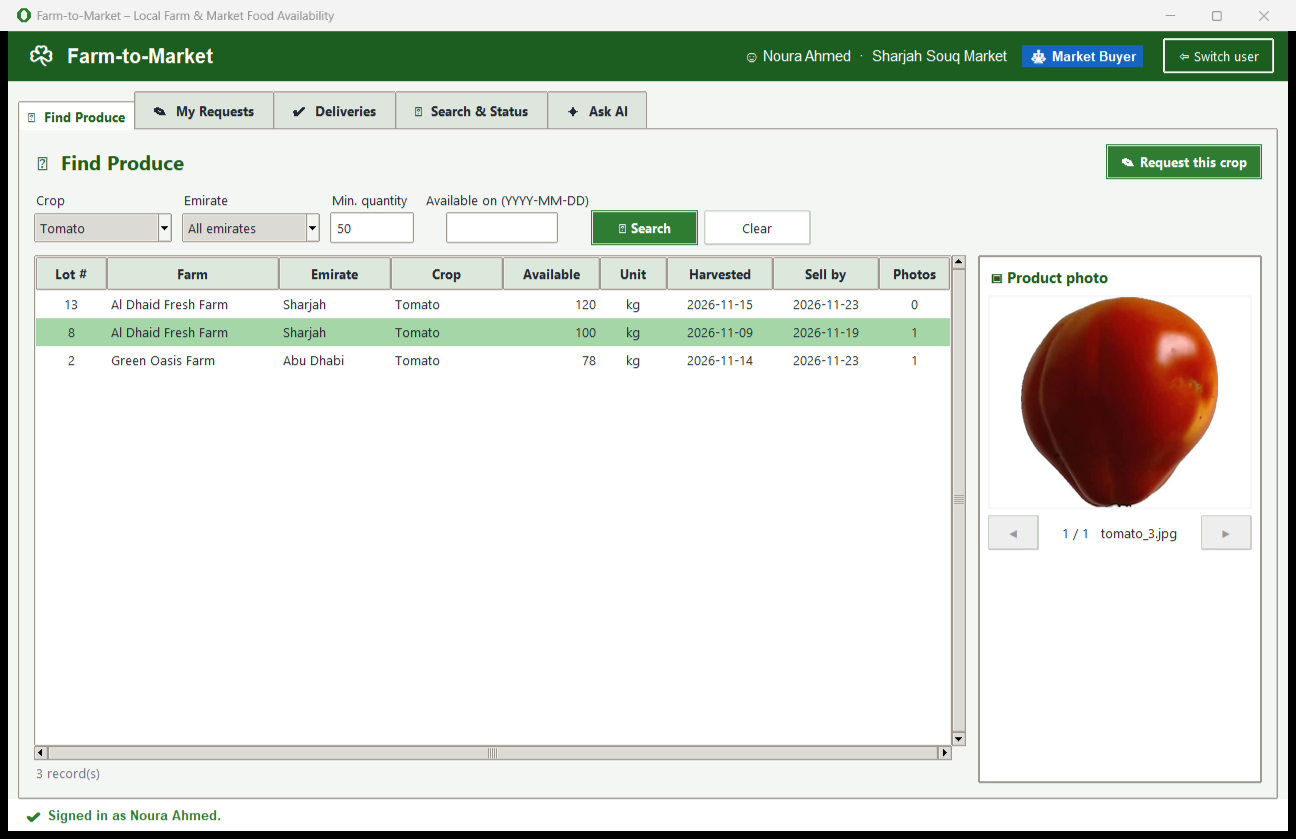
\includegraphics[width=\linewidth,height=.32\textheight,keepaspectratio]{figures/gui/search.png}
\caption{Buyer search results with availability filters and a lot photo.}
\label{gui:search}
\end{figure}
\textbf{Deliveries.} Pending allocations appear above the receipt form. The buyer enters the actual received quantity and a reason for any difference. Saved receipts show allocated, received and discrepancy quantities together.
\begin{figure}[H]\centering
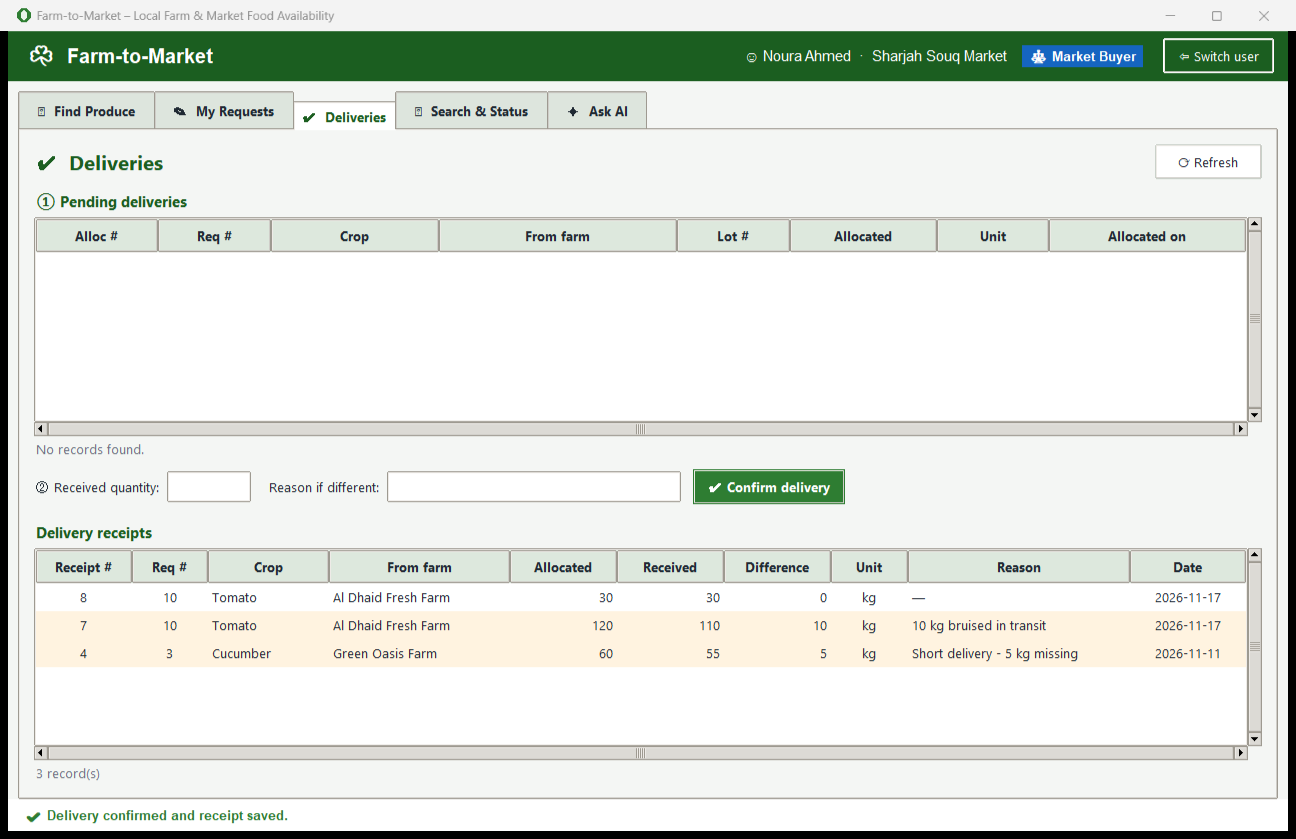
\includegraphics[width=\linewidth,height=.32\textheight,keepaspectratio]{figures/gui/delivery.png}
\caption{Buyer delivery confirmation and saved receipt discrepancies.}
\label{gui:delivery}
\end{figure}
\clearpage
\section{Loss and Surplus and the assistant}
\textbf{Loss and Surplus.} Adjustable day thresholds identify near-expiry and unallocated stock. Priority flags, available quantity, unit and sell-by date support the farmer's choice of donation or disposal; disposition history appears below.
\begin{figure}[H]\centering
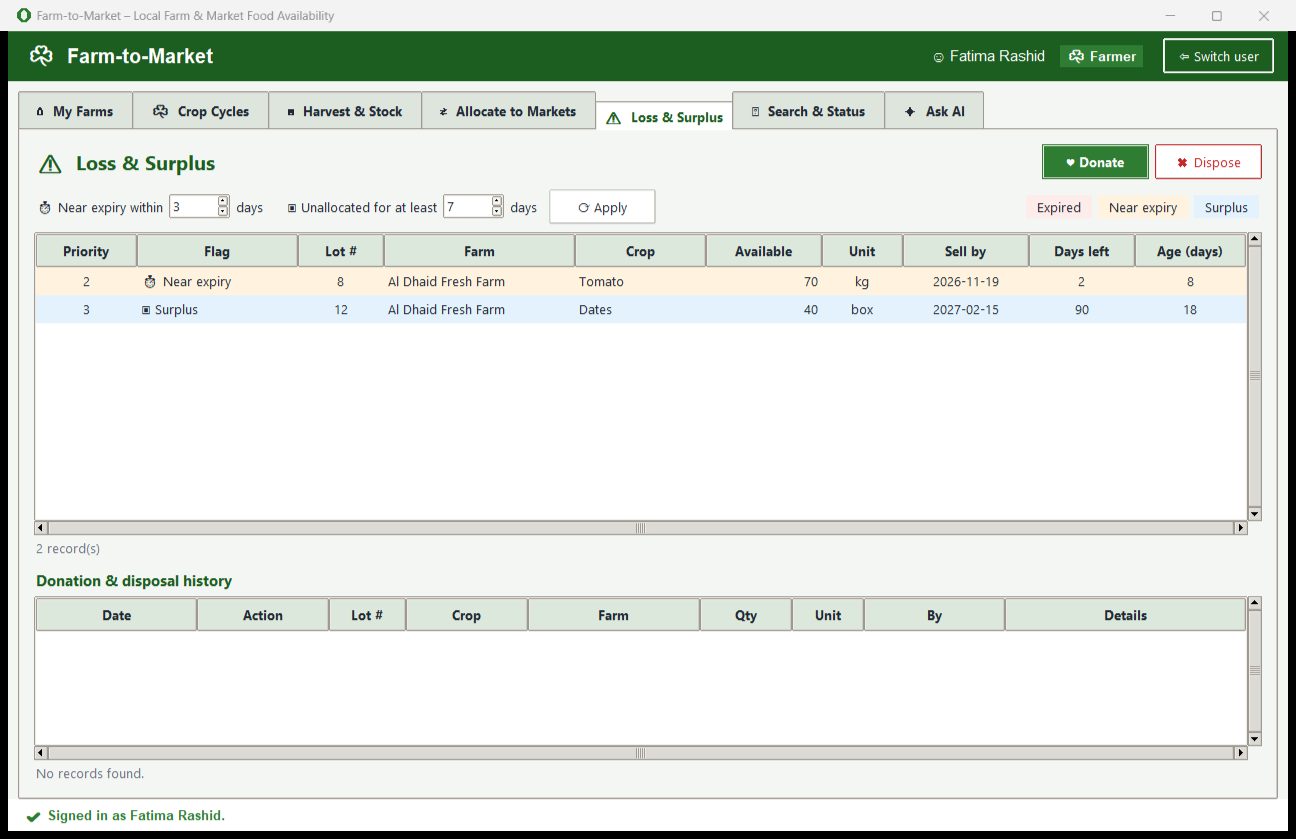
\includegraphics[width=\linewidth,height=.32\textheight,keepaspectratio]{figures/gui/surplus.png}
\caption{Loss and Surplus thresholds, candidate lots and history area.}
\label{gui:surplus}
\end{figure}
\textbf{Ask AI.} The user submits a question and receives an answer with generated SQL and supporting records. This recorded example shows a lot's on-hand, reserved and available quantities, keeping the answer directly comparable with its evidence.
\begin{figure}[H]\centering
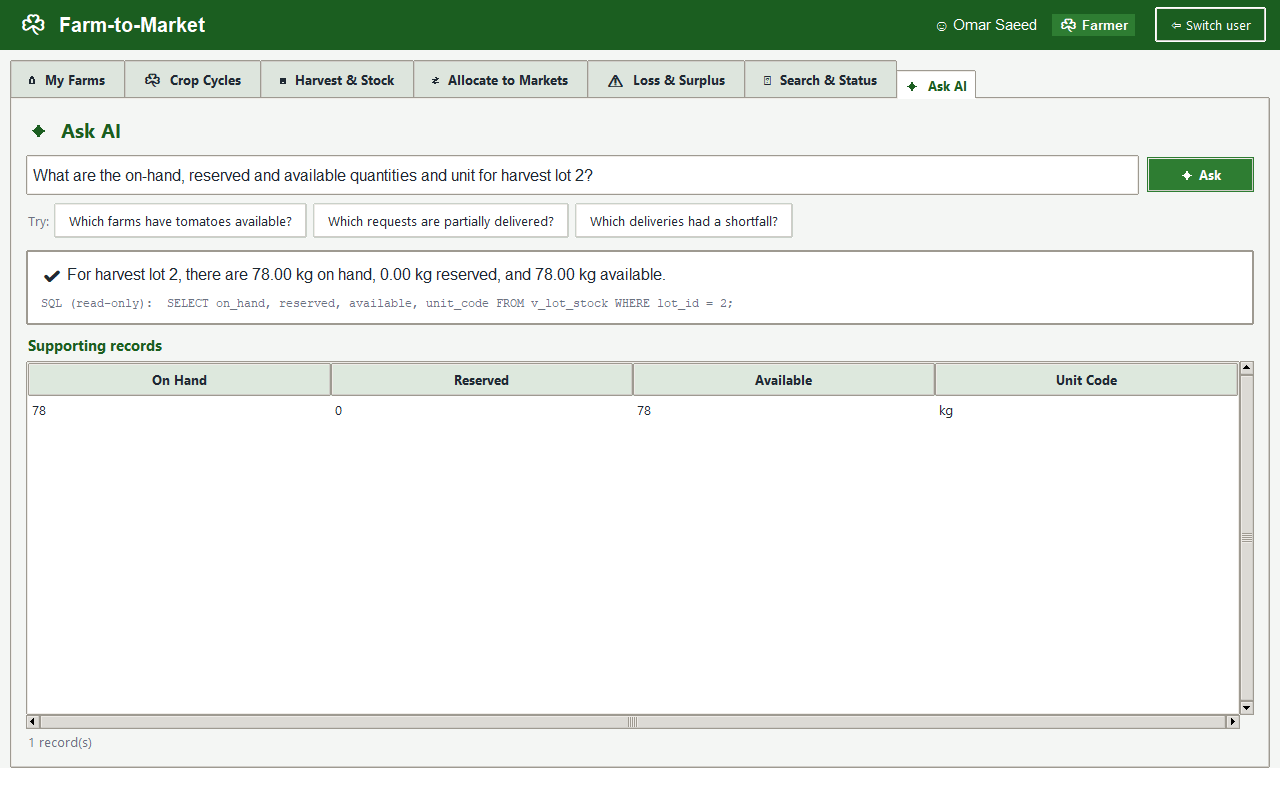
\includegraphics[width=\linewidth,height=.32\textheight,keepaspectratio]{figures/gui/assistant.png}
\caption{Assistant answer with read-only SQL and supporting quantities.}
\label{gui:assistant}
\end{figure}
\clearpage
\section{Administrator workspace}
The Users tab lists fictional accounts, roles, market membership, farm assignments and active status. Its controls support user creation, farm assignment and activation/deactivation. Reference Data maintains crops, units and markets; Activity Log supports operational review. Administrators inspect operational records without performing farmer or buyer transactions.
\begin{figure}[H]\centering
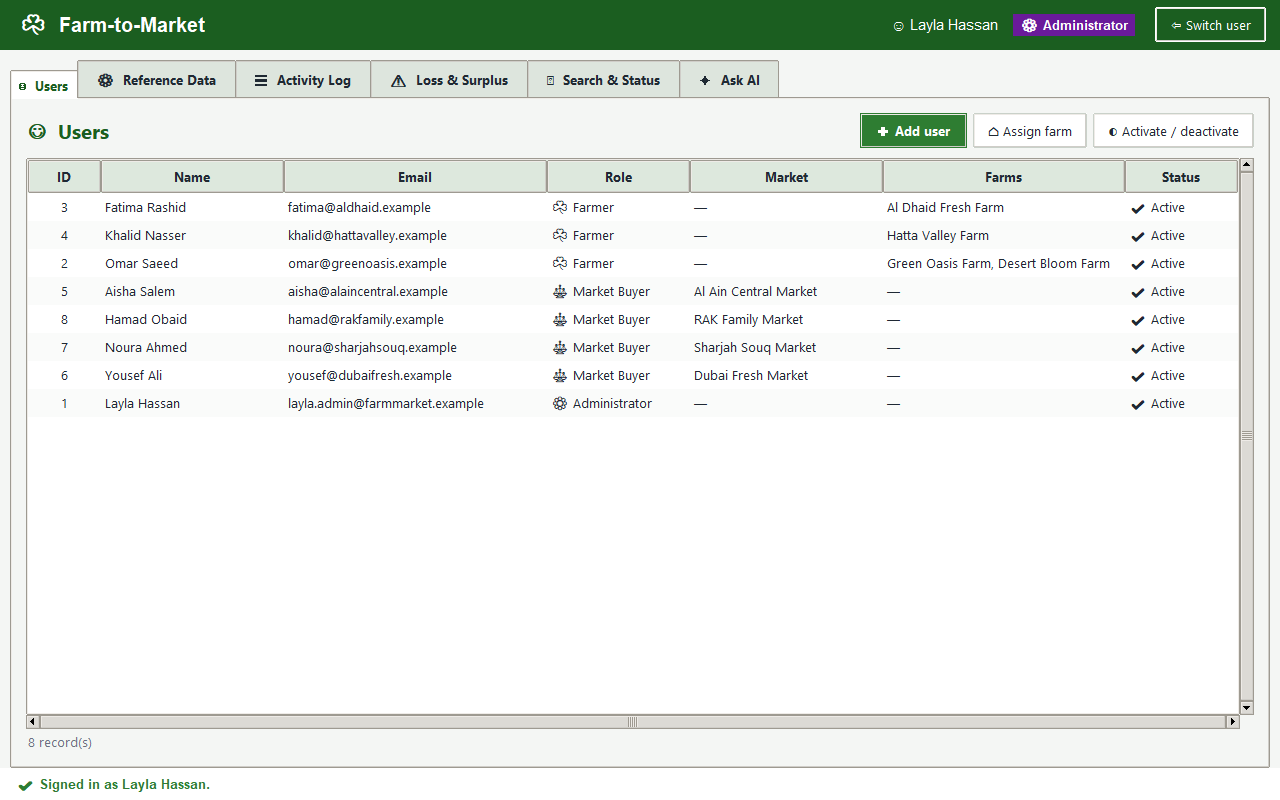
\includegraphics[width=\linewidth,height=.44\textheight,keepaspectratio]{figures/gui/admin-users-2026-11-19.png}
\caption{Administrator user management and farm/market assignments.}
\label{gui:admin-users-2026-11-19}
\end{figure}
The administrator view shows the active demo users and their existing role assignments on November 19, 2026. [R10]


\endgroup
\chapter{Verification results}
The recorded validation used Windows, Python 3.12 and MySQL 8.0.46. Expected and actual outcomes below come from November 16-17 evidence. The November 17 integrity verification recorded 173 backend checks, 22 GUI checks, seven assistant/read-only checks and the original 65-check suite. The documented donation eligibility rule is the current approved policy. [R4-R6]

\begingroup\small\setstretch{1.12}\setlength{\tabcolsep}{3pt}
\begin{longtable}{>{\raggedright\arraybackslash}p{0.43\linewidth}>{\raggedright\arraybackslash}p{0.24\linewidth}>{\raggedright\arraybackslash}p{0.25\linewidth}}
\caption{Selected expected and observed outcomes}\\\toprule
\textbf{Case and action} & \textbf{Expected} & \textbf{Observed result} \\ \midrule
\endfirsthead
\toprule
\textbf{Case and action} & \textbf{Expected} & \textbf{Observed result} \\ \midrule
\endhead
\midrule\multicolumn{3}{r}{\small Continued on next page}\\\endfoot
\bottomrule\endlastfoot
DB-01b seed counts: farms, markets, crops, cycles, lots, movements, requests, receipts & At least 3/\allowbreak{}4/\allowbreak{}5/\allowbreak{}8/\allowbreak{}12/\allowbreak{}15/\allowbreak{}8/\allowbreak{}6 & 4/\allowbreak{}4/\allowbreak{}6/\allowbreak{}10/\allowbreak{}13/\allowbreak{}38/\allowbreak{}9/\allowbreak{}6; 12 BLOB images. Pass. \\[4pt]
DB-02a-q invalid SQL constraints & Reject; no changes & 17 violations rejected; before/\allowbreak{}after checksums equal. Pass. \\[4pt]
STK-02 loss 10, correction +2 then -1 on 100 & Available 90, 92, 91 & 90, 92, 91. Pass. \\[4pt]
STK-04 add forecast 999,999 kg & Stock unchanged & On-hand/\allowbreak{}reserved/\allowbreak{}available unchanged. Pass. \\[4pt]
DEL-02 allocate 30; receive 25 from 100 & Receipt 30/\allowbreak{}25/\allowbreak{}5; final 70/\allowbreak{}0/\allowbreak{}70 & Exact receipt and balances. Pass. \\[4pt]
TX-01a-f fail after first write in six operations & Full rollback & All table checksums unchanged. Pass; injected error, not a real network outage. \\[4pt]
LS-02/\allowbreak{}03 threshold and exact-date boundaries & Valid inclusive bounds; invalid values rejected & 0/\allowbreak{}60, 0/\allowbreak{}365 and date/\allowbreak{}age boundaries behaved as expected. Pass. \\[4pt]
LS-04/\allowbreak{}05 disposition quantities and ownership & 0.01/\allowbreak{}exact available succeed; excess/\allowbreak{}unauthorized fail & Positive/exact-available quantities accepted; excess and unauthorized actions rejected in the recorded cases. \\[4pt]
GUI request, two allocations, partial receipts & 150 allocated, 140 received; discrepancy 10 & Persisted; DELIVERED under current policy. Pass as behavior observation. \\[4pt]
GUI-IMG-02 new-process photo retrieval & Same bytes and rendered photo & SHA-256 equal; photo rendered. Pass. \\[4pt]
\end{longtable}\endgroup
\section{Transaction and assistant verification}
Competing allocations, loss/correction operations and same-request releases/receipts were exercised under READ COMMITTED with explicit row locks. Recorded concurrent cases preserved the stock limits and related-record consistency. The assistant's read-only checks retained an unchanged database fingerprint; a direct write was rejected by MySQL error 1792. [R5, R6]

Fourteen recorded assistant questions covered supported stock and delivery queries, clarification, unsupported requests, protected-data refusal and empty results. Answers were compared with reference SQL or the expected response category. Generated SQL and supporting records are visible in the GUI. [R5]

\chapter{Operation and project summary}
The README supplies installation, MySQL configuration and launcher steps. Each device uses its own server and credentials in \path{app/.env}. Restarting preserves records and photos. Initial setup recreates \path{farm_market_db}; it is used when initialization or reset is intended. Live assistant answers require a Gemini key and network access.


Farm-to-Market connects farm and market workflows through movement-based stock, explicit units, ownership checks, transactions and stored photos. Loss \& Surplus records donation/disposal actions under the approved sell-by rule. The read-only assistant displays SQL and supporting records. The appendices provide the full database diagrams. Sample images carry the supplied Fruits-360 / CC BY-SA 4.0 attribution. [R8]

\section{Project poster}
Figure~\ref{fig:project-poster} summarizes the architecture, stock ledger and workflows. Its five-day threshold is a configurable example; the application default is three days.
\begin{figure}[H]\centering
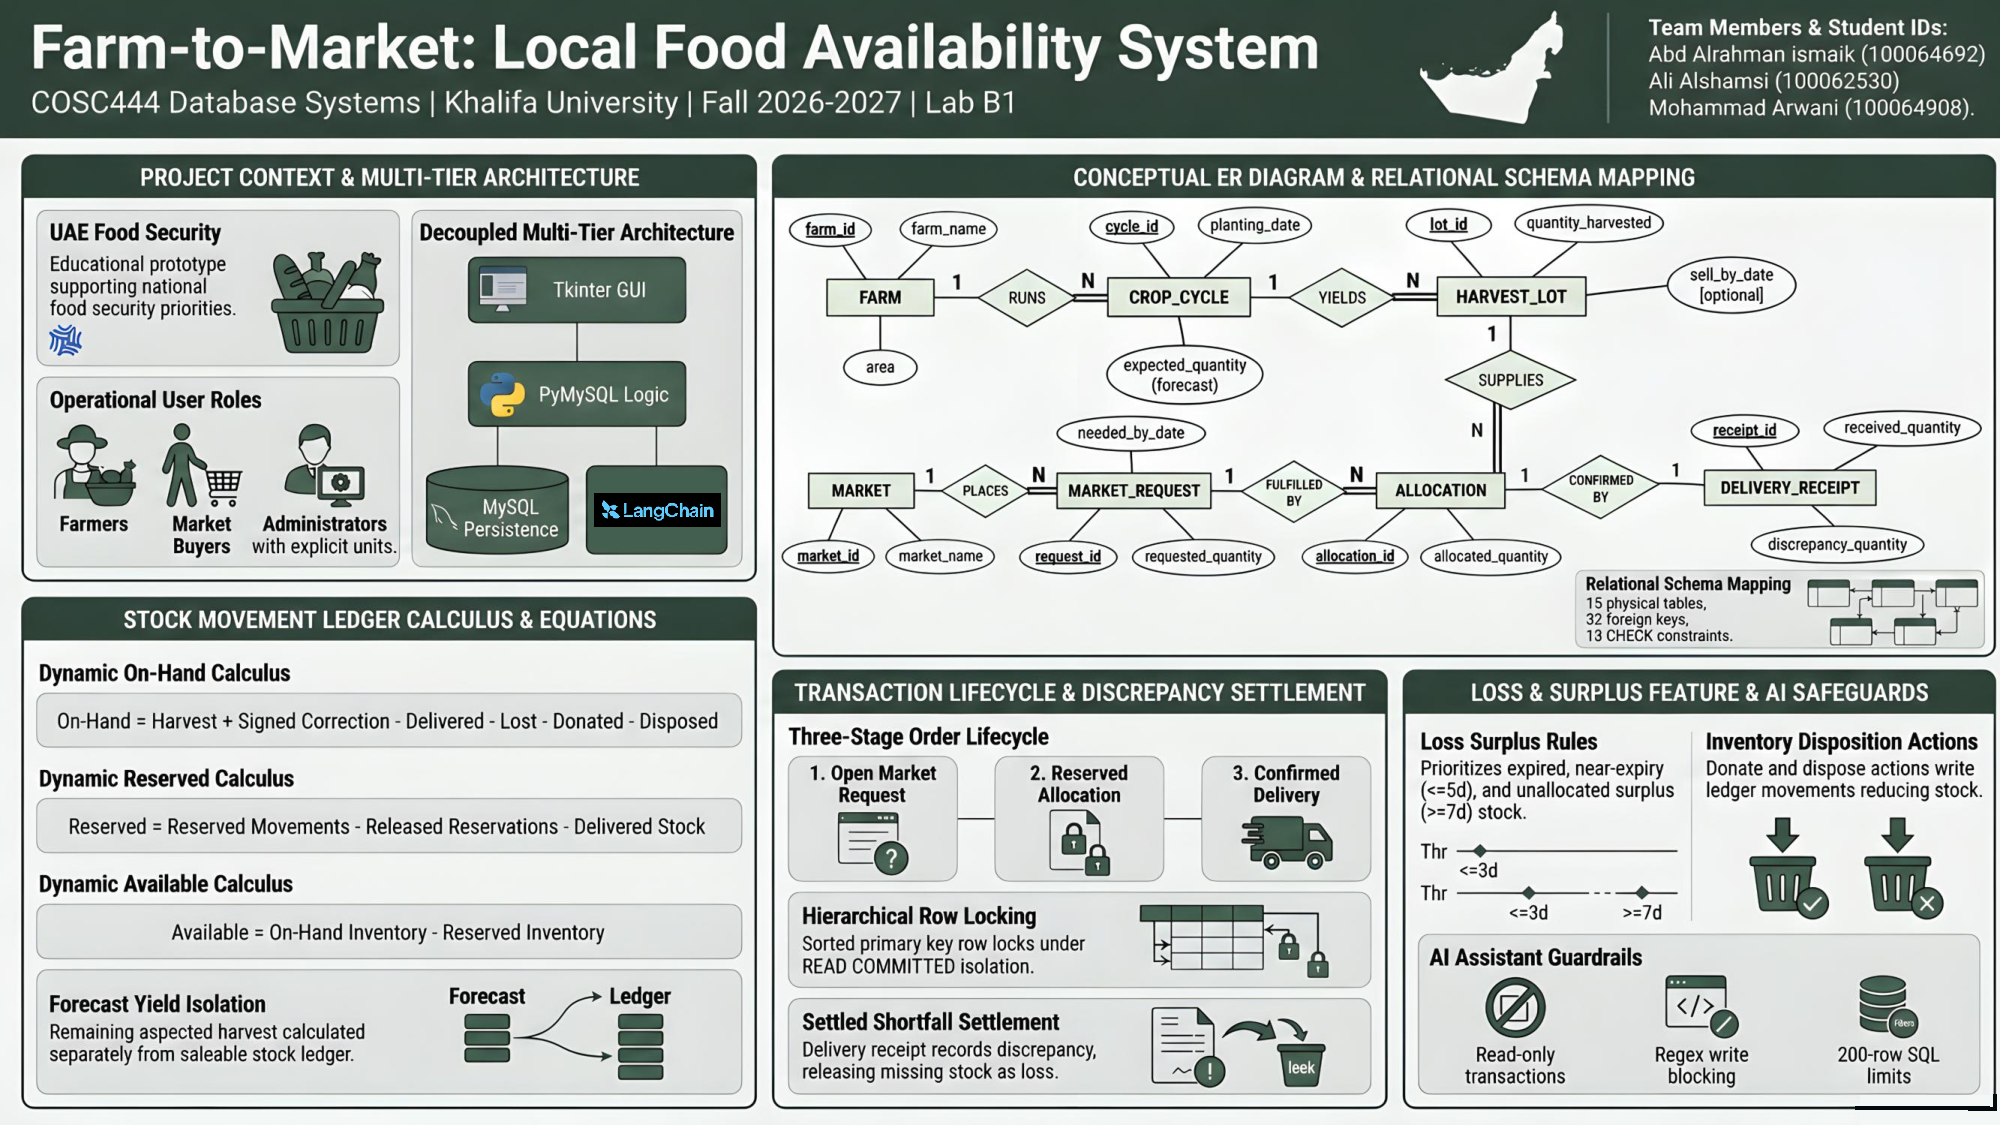
\includegraphics[width=\linewidth,height=0.38\textheight,keepaspectratio]{figures/poster.pdf}
\caption{Farm-to-Market project poster.}
\label{fig:project-poster}
\end{figure}

\chapter*{References and source versions}\addcontentsline{toc}{chapter}{References and source versions}

[R1] Original four-page proposal: \path{docs/sources/Local_Farm_Market_Food_Availability_Project_Proposal.pdf}.

[R2] Supplied \path{docs/ANNOUNCEMENTS.md}, \path{docs/PROJECT_REQUIREMENTS.md} and \path{docs/RUBRIC_AND_COVERAGE.md}; all ten rubric categories total 100, without predicted marks.

[R3] Application and database implementation: \path{app/app.py}, \path{app/db.py}, \path{app/assistant.py} and \path{app/schema.sql}.

[R4] \path{docs/evidence/VALIDATION.md}, 16 November with 17 November update; original Windows/\allowbreak{}MySQL observations and limits.

[R5] \path{docs/evidence/AI_VALIDATION.md}, \path{live-ai-initial.json}, \path{live-ai-results.json}, \path{live-ai-additional.json}, \path{gui-live-results.json}; 17 November segmented live evidence.

[R6] Database design and verification records: \path{docs/DATABASE_DESIGN.md}, \path{docs/evidence/REMAINING_TEST_RESULTS.md} and \path{docs/evidence/FIX_VALIDATION.md}.

[R7] Operating guide and team information: \path{docs/DEMO_AND_SUBMISSION.md} and \path{docs/TEAM.md}.

[R8] \path{docs/IMAGE_ATTRIBUTION.md}; upstream \href{https://github.com/fruits-360/fruits-360-original-size/blob/main/README.md}{Fruits-360 original-size README} and \href{https://github.com/fruits-360/fruits-360-original-size/blob/main/LICENSE}{license}, checked 17 November 2026; local asset inventory and attribution notes supplied.


[R9] Startup and configuration: root \path{README.md}, \path{run.bat}, \path{app/run.bat} and \path{app/check_database.py}.


[R10] GUI screenshots: preserved application captures in \path{docs/evidence/}; administrator Users view captured November 19, 2026 using read-only database sessions. The figure asset inventory records source paths and dates.

\appendix
\chapter{Conceptual ER diagrams}
The five figures retain the original conceptual model: two entity-attribute sheets followed by three relationship sheets. Each source sheet is embedded as a vector figure with its original proportions; the report keeps standard A4 page dimensions. [R6]

\begin{figure}[htbp]\centering
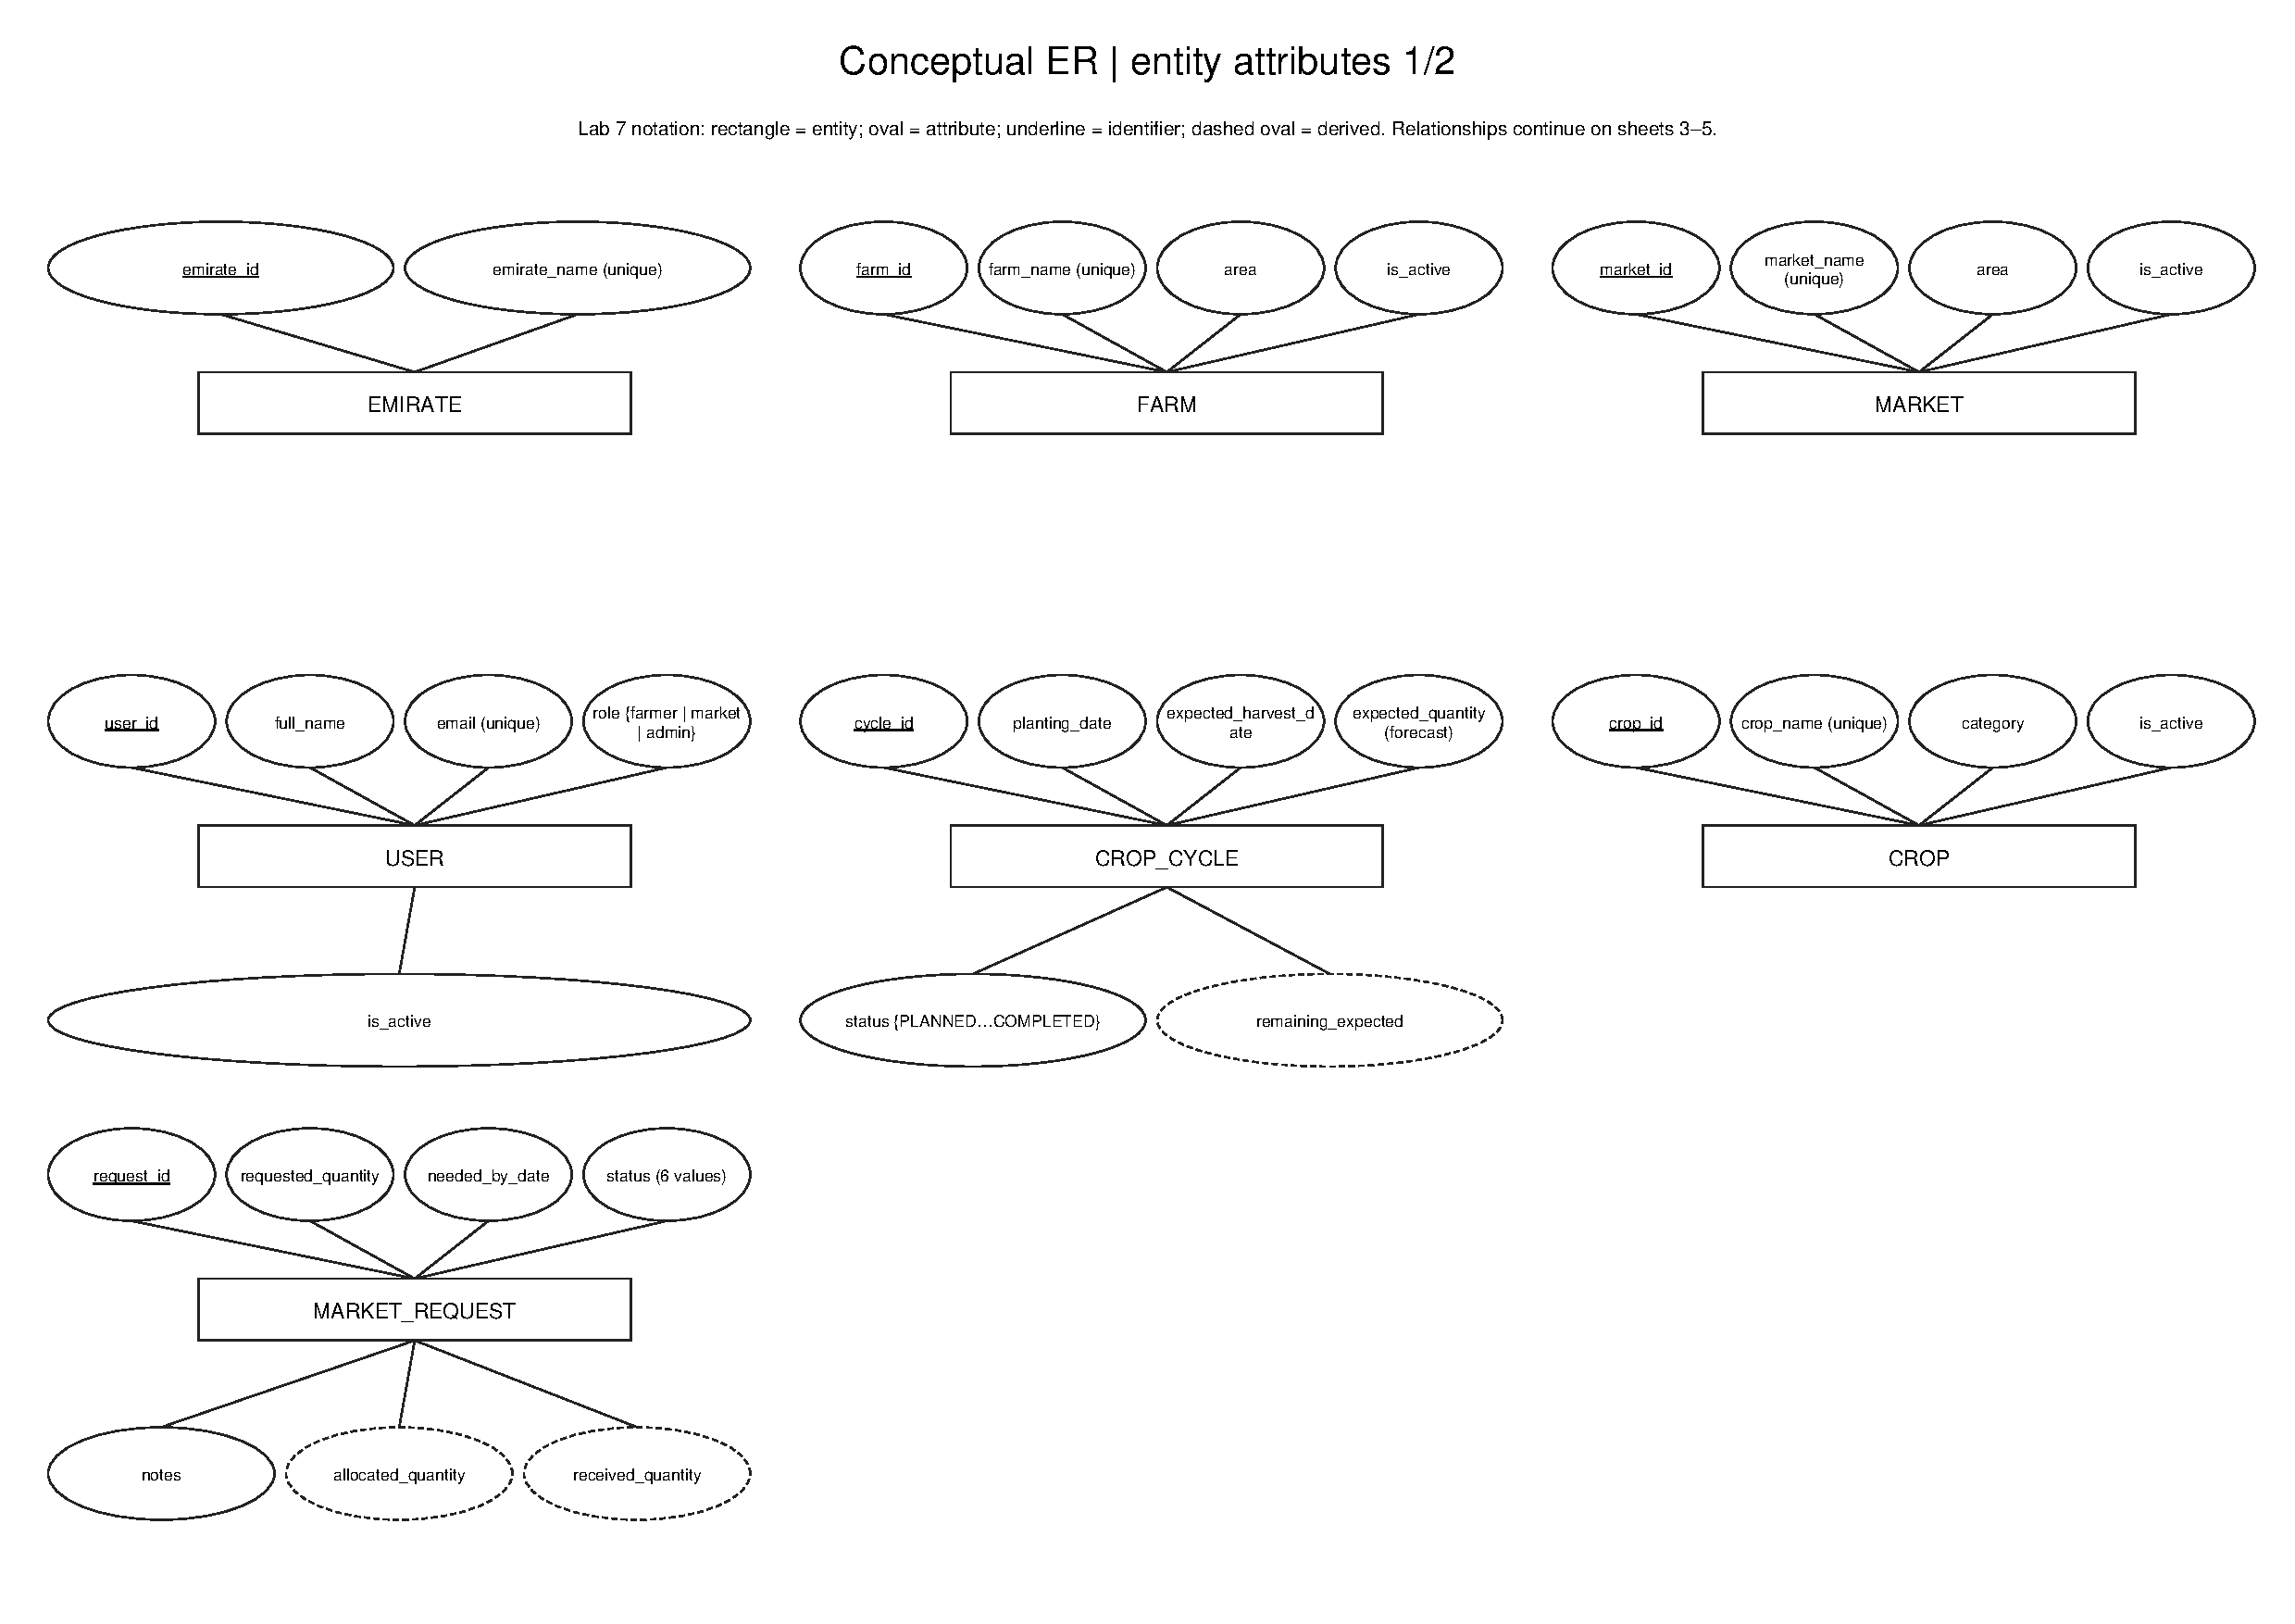
\includegraphics[page=1,width=\linewidth,height=0.42\textheight,keepaspectratio]{figures/conceptual-er.pdf}
\caption{Conceptual ER model: entity attributes, sheet 1 of 2.}
\label{fig:conceptual-er-1}
\end{figure}

\begin{figure}[htbp]\centering
\includegraphics[page=2,width=\linewidth,height=0.42\textheight,keepaspectratio]{figures/conceptual-er.pdf}
\caption{Conceptual ER model: entity attributes, sheet 2 of 2.}
\label{fig:conceptual-er-2}
\end{figure}

\begin{figure}[htbp]\centering
\includegraphics[page=3,width=\linewidth,height=0.42\textheight,keepaspectratio]{figures/conceptual-er.pdf}
\caption{Conceptual ER model: relationships, sheet 1 of 3.}
\label{fig:conceptual-er-3}
\end{figure}

\begin{figure}[htbp]\centering
\includegraphics[page=4,width=\linewidth,height=0.42\textheight,keepaspectratio]{figures/conceptual-er.pdf}
\caption{Conceptual ER model: relationships, sheet 2 of 3.}
\label{fig:conceptual-er-4}
\end{figure}

\begin{figure}[htbp]\centering
\includegraphics[page=5,width=\linewidth,height=0.42\textheight,keepaspectratio]{figures/conceptual-er.pdf}
\caption{Conceptual ER model: relationships, sheet 3 of 3.}
\label{fig:conceptual-er-5}
\end{figure}
\chapter{Relational schema diagrams}
The three figures retain all fifteen original relations, attributes, keys, types and constraints. The source exports are embedded unchanged as vector figures within standard A4 report pages. The executable DDL remains in \path{app/schema.sql}. [R3, R6]

\begin{figure}[htbp]\centering
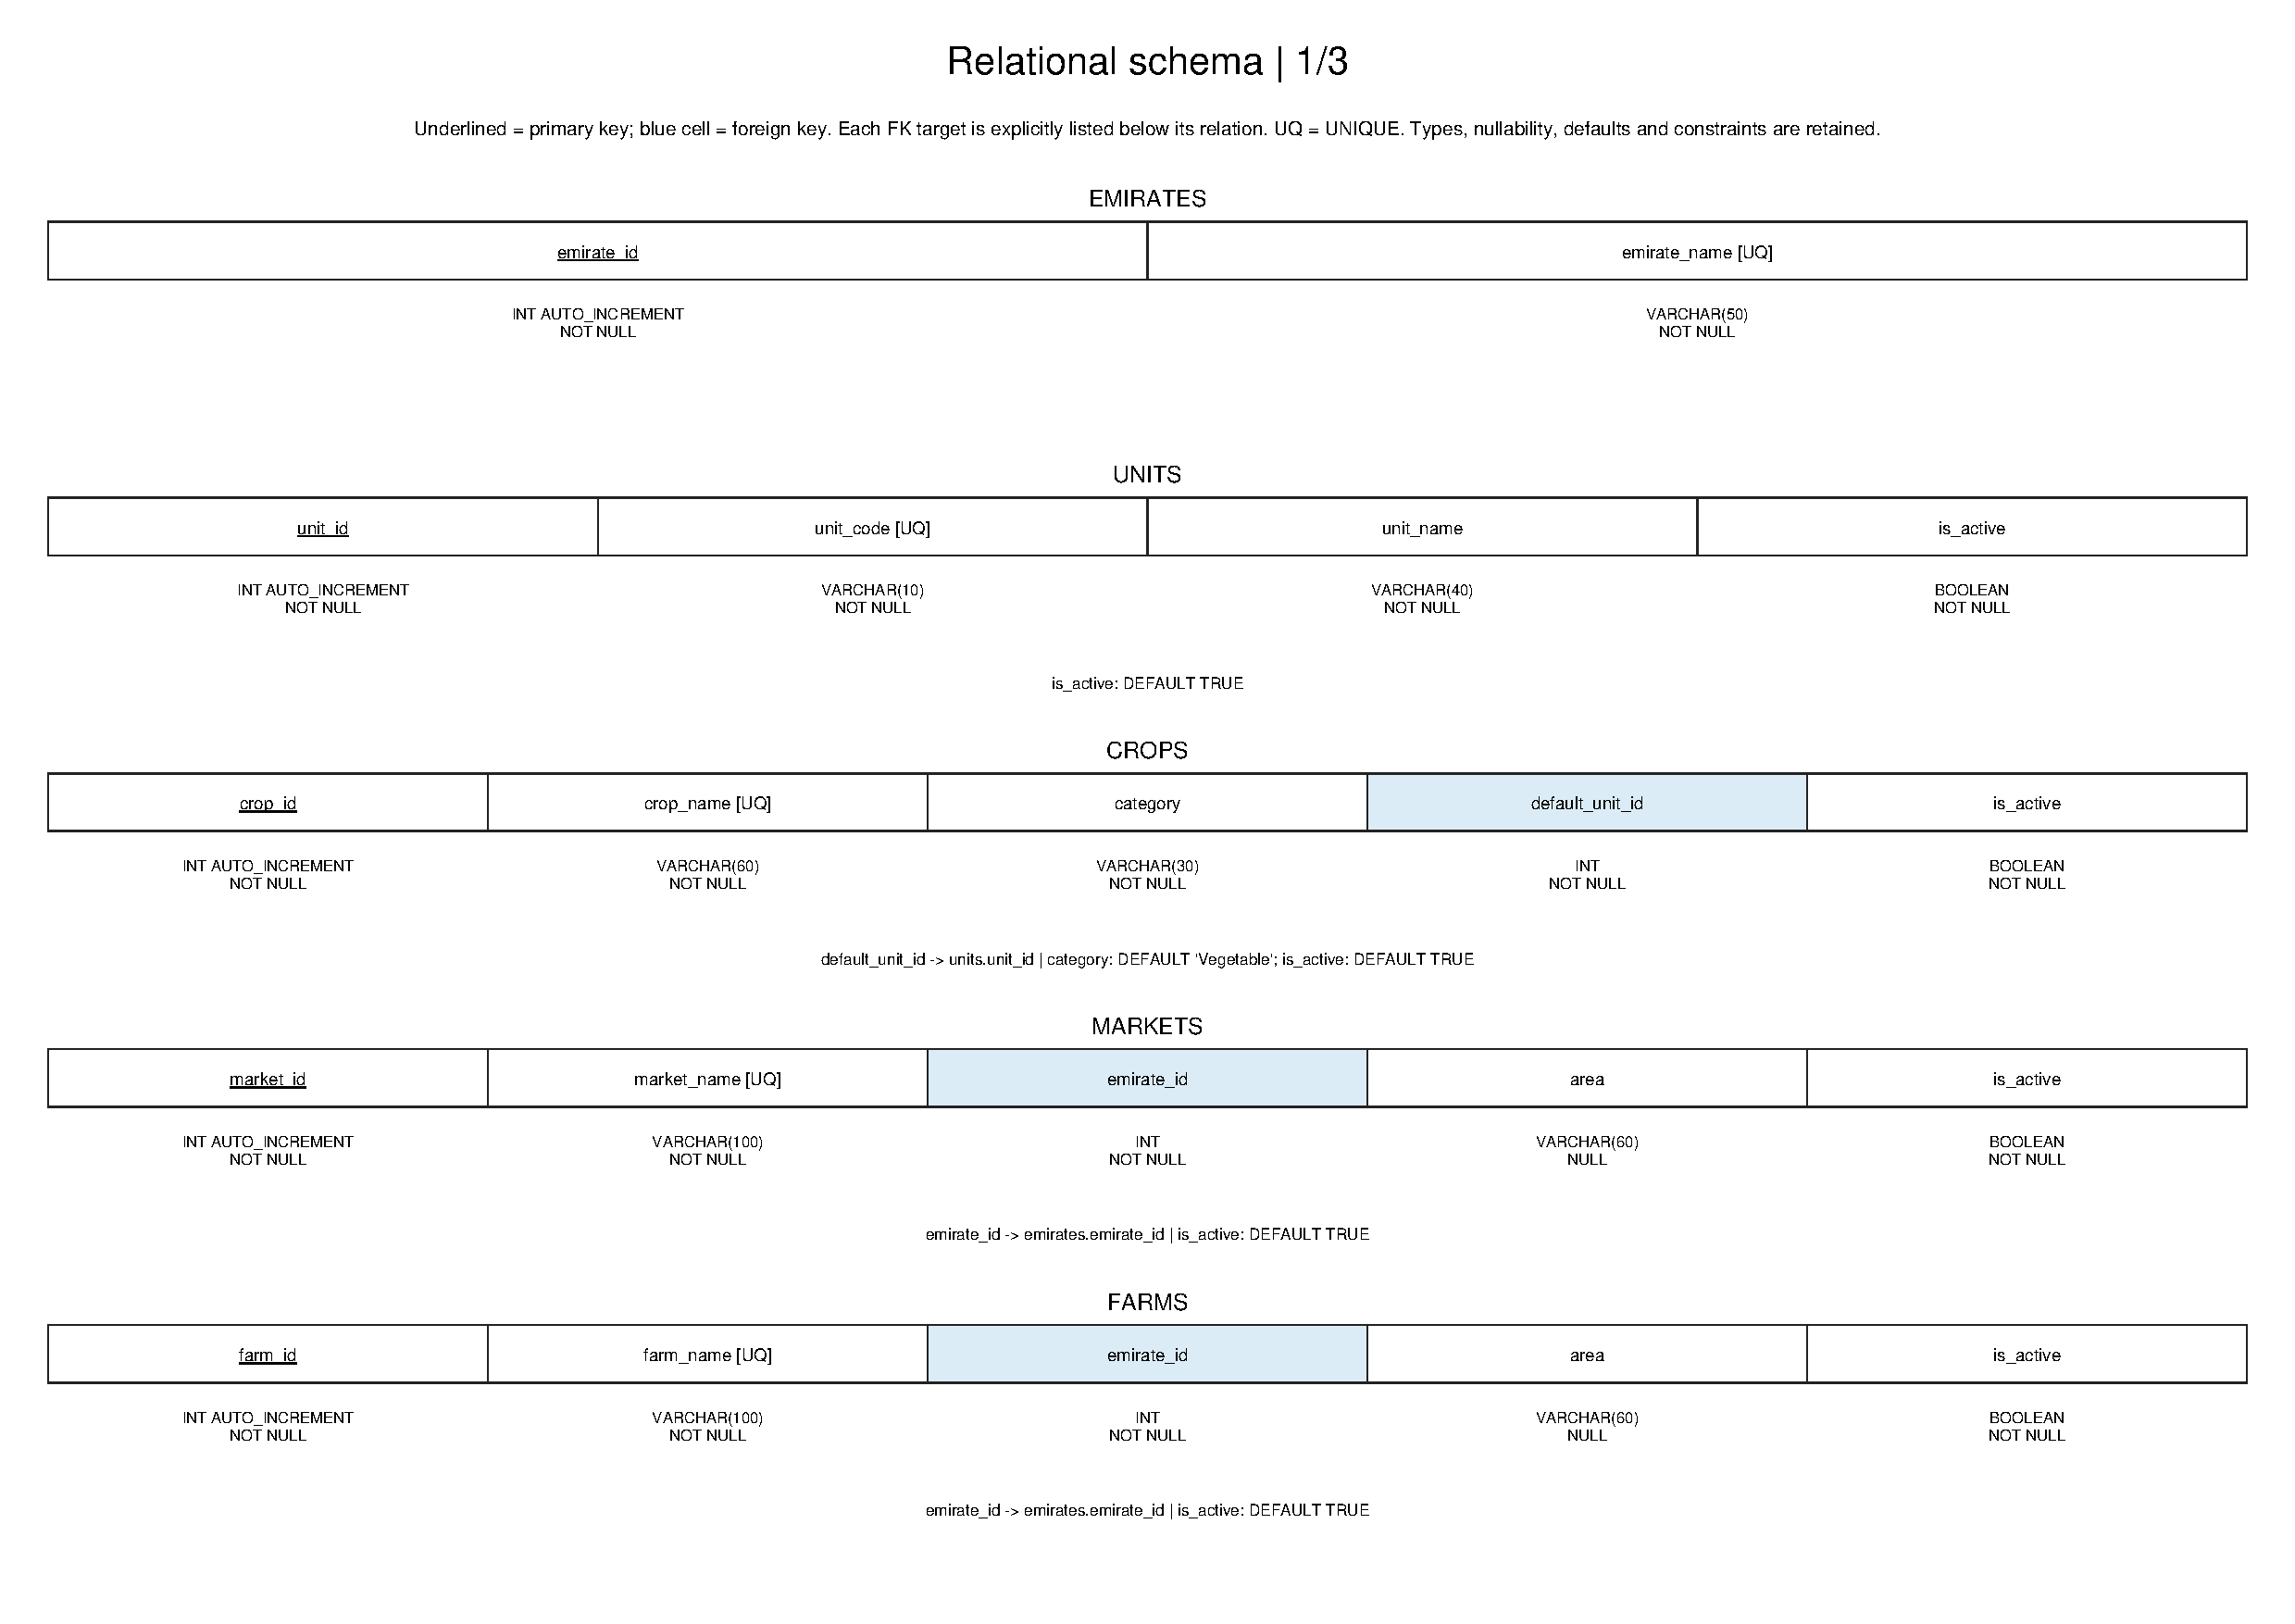
\includegraphics[page=1,width=\linewidth,height=0.42\textheight,keepaspectratio]{figures/relational-schema.pdf}
\caption{Relational schema, sheet 1 of 3.}
\label{fig:relational-schema-1}
\end{figure}

\begin{figure}[htbp]\centering
\includegraphics[page=2,width=\linewidth,height=0.42\textheight,keepaspectratio]{figures/relational-schema.pdf}
\caption{Relational schema, sheet 2 of 3.}
\label{fig:relational-schema-2}
\end{figure}

\begin{figure}[htbp]\centering
\includegraphics[page=3,width=\linewidth,height=0.42\textheight,keepaspectratio]{figures/relational-schema.pdf}
\caption{Relational schema, sheet 3 of 3.}
\label{fig:relational-schema-3}
\end{figure}
\end{document}
